\def\fileversion{v1.0n} \def\filedate{2009/4/23}
\documentclass[12pt,oneside]{book}
\usepackage[fullpage]{uiucthesis}

%\usepackage[fullpage,draftthesis]{uiucthesis}
%\def\draftheader{\slshape Preliminary Examination Document}


%\usepackage{graphicx}
%\usepackage{times}
%\usepackage{psfrag}
%\usepackage{psfig}
%\usepackage{epsfig}
%\usepackage{latexsym, amsmath, amsfonts, amscd}
%\usepackage{hhline,multirow}
%\usepackage{fancyhdr}
%\usepackage{pifont}\usepackage{array}

% This is required for dvipdfm
%\usepackage[dvipdfm]{color}
%
% graphicx.sty has some useful transformation features not present in 
% graphics.sty
%\usepackage[dvipdfm]{graphicx}
\usepackage{graphicx}
%
% natbib.sty has many features for a variety of citation styles.  Remember 
% to use \citep!
% use "sort&compress" for newer versions of natbib, "sort" for older versions
%\usepackage[square,sort&compress]{natbib}
%
% This makes many more AMS math symbols available.
\usepackage{amsmath}
\usepackage{amssymb}

% array.sty and dcolumn.sty extend the features of the tabular and array 
% environments.  
\usepackage{dcolumn,array}

\usepackage{cite}
\usepackage{times}
\usepackage{fancyhdr}
\usepackage{float}
\usepackage{psfrag}
%\usepackage{psfig}
\usepackage{subfigure}
\usepackage{epsfig}
\usepackage{latexsym,amsfonts,amsthm,amscd}
\usepackage{algorithm}
\usepackage{algorithmic}
\usepackage{cmmib57}
\usepackage{pifont}
%\usepackage{bibmods}\usepackage{bibnames}
\usepackage{makeidx}
\usepackage[noprefix]{nomencl}
\usepackage{hhline,multirow}

\usepackage{url}

%\usepackage{graphicx}

%
% Using those packages, one can define these new column types:
\newcolumntype{.}{D{.}{.}{-1}}
\newcolumntype{d}[1]{D{.}{.}{#1}}
%
% hyperref works, but not quite like I'd want 
% The main problem is that it does not currently handle \addcontentsline
% which we *do* use below!
% Perhaps in the future this will be ironed out.
% Leave this commented out for now.
% \usepackage[dvipdfm]{hyperref}
% 
% The following two packages, epic.sty and eepic.sty, allow xfig output 
% to be rendered (nicely) by TeX.  
\usepackage{epic}
\usepackage{eepic}

%  
% The ifthen.sty package is useful for setting up switches for things like
% color/grayscale images, compact formatting, etc.  
\usepackage{ifthen}
%
% mydefs.sty is where to place customized definitions.   
\usepackage{mydefs}

\usepackage[usenames]{color}

% Hopefully get psfrag to work
%\usepackage{psfrag}

% Set page dimensions.

\textheight=8.4in
\headheight=0pt
\headsep=0pt
\topmargin=0.1in
\textwidth=6.3in
\oddsidemargin=0.1in
%\evensidemargin=0.0in

\setlength\fboxsep{0pt}
\setlength\fboxrule{1pt}

%\newcommand{\ind}{\hspace{\parindent}}
\newcommand{\simgt}{$>$\hspace{-9pt}\raisebox{-6pt}{$\sim$}\ }
\newcommand{\simlt}{$<$\hspace{-9pt}\raisebox{-6pt}{$\sim$}\ }

\newcommand{\ie}{{i.e.}}
\newcommand{\D}{\displaystyle}
\newenvironment{principle}[1][Principle]{\begin{trivlist} \item[\hskip \labelsep {\bfseries #1}] \em }{\end{trivlist}}
\newtheorem{theorem}{Theorem}[chapter]
\newtheorem{example}{Example}[chapter]
\newtheorem{definition}{Definition}[chapter]
\newtheorem{proposition}{Proposition}[chapter]
\newtheorem{Principle}{Principle}[chapter]
\def\QED{~\rule[-1pt]{5pt}{5pt}\par\medskip}
\newenvironment{proof}{{\bf Proof: \ }}{ \hfill \QED}

\newcommand{\p}{{p}}
\renewcommand{\Re}{{\mathbb{R}}}
\newcommand{\Ze}{{\mathbb{Z}}}
\newcommand{\Pe}{{\mathbb{P}}}
\renewcommand{\Im}{\mathcal{I}}
\def\X{{\boldsymbol{X}}}
\def\x{{\boldsymbol{x}}}
\def\Y{{\boldsymbol{Y}}}
\def\y{{\boldsymbol{y}}}
\def\F{{\mathbf{F}}}

% procedural macros:
\newcommand{\be}{\begin{equation}}
\newcommand{\ee}{\end{equation}}
\newcommand{\bea}{\begin{eqnarray}}
\newcommand{\eea}{\end{eqnarray}}

% variable macros:
\newcommand{\lp}{\left(}
\newcommand{\rp}{\right)}
\newcommand{\lb}{\left[}
\newcommand{\rb}{\right]}

\newcommand{\au}{ ^{197}{\rm Au} }
\newcommand{\avgpx}{\langle p_{x}(y) \rangle}
\newcommand{\avgpxpp}{\langle p_{x} / p_{\bot} \rangle}
\newcommand{\avgm}{\langle M_{c}(b) \rangle}
\newcommand{\avgteff}{\langle \Theta_{\rm eff}(\beta,E) \rangle}
\newcommand{\avgtf}{\langle \theta_{\rm F}(b) \rangle}
\newcommand{\bimp}{b}
\newcommand{\betamax}{\beta_{\rm max}}
\newcommand{\crosssect}{\sigma({\bf p},{\bf p'}\leftrightarrow{\bf q},{\bf q'})}
\newcommand{\dt}{\Delta t}
\newcommand{\ebal}{E_{\rm bal}}
\newcommand{\ecm}{E_{\rm cm}}
\newcommand{\elab}{E_{\rm lab}}
\newcommand{\ep}{E_{\rm P}}
\newcommand{\erho}{E(\rho)}
\newcommand{\es}{E_{\rm S}}
\newcommand{\f}[1]{f \lp {\bf #1},{\bf r} \rp}
\newcommand{\flow}{{\cal F}}
\newcommand{\fpr}{f \lp {\bf p},{\bf r} \rp}
\newcommand{\fprt}{f \lp {\bf p},{\bf r}, t \rp}
\newcommand{\gradr}{ \mbox{\boldmath $\nabla\!$}_{r}}
\newcommand{\gradp}{ \mbox{\boldmath $\nabla\!$}_{p}}
\newcommand{\la}{ ^{139}{\rm La} }
\newcommand{\lam}[1]{\lambda_{#1}}
\newcommand{\mc}{M_{c}}
\newcommand{\mclimit}{M_{c}^{\rm limit}}
\newcommand{\mcmax}{M_{c}^{\rm max}}
\newcommand{\mua}{\mu_{\rm a}}
\newcommand{\mur}{\mu_{\rm r}}
\newcommand{\mult}{\langle M \rangle}
\newcommand{\multb}{\langle M(\bimp) \rangle}
\newcommand{\np}{N_{p}}
\newcommand{\npmax}{N_{p}^{\rm max}}
\newcommand{\nscat}{N_{\rm scat}}
\newcommand{\ntest}{N_{\rm test}}
\newcommand{\ppar}{\left( {\bf p} \right)}
\newcommand{\pxn}{\langle p_{x}(v_{z}) \rangle}
\newcommand{\qvec}{{\bf Q}}
\newcommand{\ralpha}{{\bf r}_{\alpha}}
\newcommand{\rc}{r_{\rm c}}
\newcommand{\rhoac}{\rho_{\rm ac}}
\newcommand{\rhobar}{\frac{\rho}{\rhoz}}
\newcommand{\rhocrit}{\rho_{\rm C}}
\newcommand{\rhoi}{\rho_{i}}
\newcommand{\rhol}{\rho_{\rm L}}
\newcommand{\rhor}{\rho \left( {\bf r} \right)}
\newcommand{\rhoz}{\rho _{0}}
\newcommand{\rhs}{r_{\rm hs}}
\newcommand{\rmin}{r_{\rm min}}
\newcommand{\rpmin}{r'_{\rm min}}
\newcommand{\rpar}{\left( {\bf r} \right)}
\newcommand{\seff}{\sigma_{\rm eff}}
\newcommand{\seffnn}{\sigma_{\rm eff, nn}}
\newcommand{\seffnp}{\sigma_{\rm eff, np}}
\newcommand{\shs}{\sigma_{\rm hs}}
\newcommand{\shsnn}{\sigma_{\rm hs, nn}}
\newcommand{\shsnp}{\sigma_{\rm hs, np}}
\newcommand{\tac}{T_{\rm ac}}
\newcommand{\tapp}{T_{\rm app}}
\newcommand{\taueff}{\tau_{\rm eff}}
\newcommand{\tcrit}{T_{\rm C}}
\newcommand{\tf}{\theta_{\rm F}}
\newcommand{\tfb}{\theta_{\rm F}(\bimp)}
\newcommand{\teffbe}{\Theta(\beta,E)}
\newcommand{\teffnnbe}{\Theta_{\rm nn}(\beta,E)}
\newcommand{\teffnpbe}{\Theta_{\rm np}(\beta,E)}
\newcommand{\ths}{\Theta_{\rm hs}(\beta)}
\newcommand{\ti}{T_{i}}
\newcommand{\tint}{T_{\rm int}}
\newcommand{\tmax}{t_{\rm max}}
\newcommand{\up}{U_{\rm P}}
\newcommand{\ur}{U \lp {\bf r} \rp}
\newcommand{\urho}{U \lp \rho \rp}
\newcommand{\us}{U_{\rm S}}
\newcommand{\va}{v_{\rm a}}
\newcommand{\vecp}{{\bf p}}
\newcommand{\vecr}{{\bf r}}
\newcommand{\veff}{v_{\rm eff}}
\newcommand{\veffnp}{v_{\rm eff,np}}
\newcommand{\veffnn}{v_{\rm eff,nn}}
\newcommand{\vk}{{\bf k}}
\newcommand{\vnp}{v_{\rm np}}
\newcommand{\vnn}{v_{\rm nn}}
\newcommand{\vpp}{v_{\rm pp}}
\newcommand{\vr}{v_{\rm r}}
\newcommand{\yproj}{y_{\rm proj}}
\newcommand{\yuk}[1]{e^{- \mu_{\rm #1} r} /r}
\newcommand{\yukc}[1]{e^{- \mu_{\rm #1} \rc} / \rc}

%frank's definitions
\newtheorem{wilbur}{Proposition}

\newcommand{\he}{$^{3}{\rm He}$--A}
\newcommand{\hel}{$^{3}{\rm He}$}
\newcommand{\heAA}{$^{3}{\rm He}$--A1}
\newcommand{\heB}{$^{3}{\rm He}$--B}

\newcommand{\nqp}{Nambu quasi-particle}
\newcommand{\lqp}{Landau quasi-particle}
\newcommand{\io}{intrinsic orbital angular momentum}
\newcommand{\am}{IOAM}
\newcommand{\fcur}{fermion number current}

\newcommand{\delo}{\mbox{${\bf \Delta}_{1}$}}
\newcommand{\delt}{\mbox{${\bf \Delta}_{2}$}}
\newcommand{\phat}{\mbox{$\hat{\mbox{\boldmath $p$}}$}}
\newcommand{\pphi}{\mbox{$\phi_{p}$}}
\newcommand{\bk}{{\bf k}}
\newcommand{\bp}{{\bf p}}
\newcommand{\bpp}{\mbox{${\bf p}^{\prime}$}}
\newcommand{\bq}{{\bf q}}
\newcommand{\bkp}{\mbox{${\bf k}^{\prime}$}}
\newcommand{\lv}{\mbox{$\hat{{\bf l}}$}}
\newcommand{\rrc}{{\rm c}}
\newcommand{\bep}{\mbox{\boldmath $\epsilon$}}
\newcommand{\bxx}{{\bf x}}
\newcommand{\byy}{{\bf y}}
\newcommand{\eps}{\mbox{$\epsilon$}}
\newcommand{\xp}{\mbox{$x^{\prime}$}}
\newcommand{\bxp}{\mbox{${\bf x^{\prime}}$}}
\newcommand{\brr}{{\bf R}}
\newcommand{\bsg}{\mbox{\boldmath $\sigma$}}
\newcommand{\bnh}{\mbox{$\hat{{\bf n}}$}}
\newcommand{\bnhp}{\mbox{$\hat{{\bf n}}_{\bf p}$}}
\newcommand{\bbb}{{\bf B}}
\newcommand{\cp}{\mbox{$C_{{\bf p}}$}}
\newcommand{\spp}{\mbox{$S_{{\bf p}}$}}


\newcommand{\cl}{\mbox{${\cal L}$}}
\newcommand{\cm}{{\cal M}}
\newcommand{\ccm}{\mbox{${\cal C}^{\mu}$}}

\newcommand{\parj}{\mbox{$^{j}_{3}\rpp$}}
\newcommand{\park}{\mbox{$^{k}_{3}\rpp$}}
\newcommand{\parl}{\mbox{$^{l}_{3}\rpp$}}

\newcommand{\rh}{\mbox{{\rm H}}}
\newcommand{\rhzp}{\mbox{${\rm H}^{\prime}_{0}$}}
\newcommand{\rhz}{\mbox{${\rm H}_{0}$}}
\newcommand{\rhc}{\mbox{${\rm H}_{\chi}$}}
\newcommand{\rhph}{\mbox{${\rm H}_{\phi}$}}
\newcommand{\rhint}{\mbox{${\rm H}_{{\rm int}}$}}
\newcommand{\rhintp}{\mbox{${\rm H}_{{\rm int}}^{\prime}$}}
\newcommand{\rs}{{\rm s}}
\newcommand{\rsp}{{\rm s}^{\prime}}

\newcommand{\vp}{^{\prime}}

\newcommand{\rpp}{{\rm P}}
\newcommand{\rt}{{\rm T}}
\newcommand{\hop}{H(\phat)}

\newcommand{\gft}{\mbox{${\rm G}_{0 \rs}(\bp,{\rm t})$}}
\newcommand{\gfp}{\mbox{${\rm G}_{0 \rs}(\bp,{\rm p}_{0})$}}
\newcommand{\gfpp}{\mbox{${\rm G}_{0}(\bpp,{\rm p}^{\prime}_{0})$}}
\newcommand{\lla}{\mbox{$\langle$}}
\newcommand{\ra}{\mbox{$\rangle$}}
\newcommand{\parr}{\mbox{$\partial$}}
\newcommand{\epar}{\mbox{$\bar{\partial}$}}
\newcommand{\gamb}{\mbox{$\bar{\gamma}$}}
\newcommand{\gamfb}{\mbox{$\bar{\gamma_{5}}$}}
\newcommand{\abar}{\mbox{$\bar{A}$}}
\newcommand{\lag}{\mbox{${\cal L}(\phat)$}}
\newcommand{\gm}{\mbox{$\gamma^{\mu}$}}
\newcommand{\dm}{\mbox{$\partial_{\mu}$}}
\newcommand{\gfiv}{\mbox{$\gamma_{5}$}}


\begin{document}

%!TEX root = thesis.tex

% TITLE.TEX:    LaTex file to produce title page for UIUC Physics
%               Department PhD Thesis
% Author: Patrick Dreher
% Date:   8/27/91

% copyright page
\renewcommand\maketitle{
  \thispagestyle{empty}
  %We need do determine TitleBoxHeight=1.75in-the height of capital letters.
  \newlength{\TitleBoxHeight}\settoheight{\TitleBoxHeight}{THESIS}
  \setlength{\TitleBoxHeight}{-1.0\TitleBoxHeight}
  \addtolength{\TitleBoxHeight}{1.75in}
  %
  %Start from 0.75in top margin
  %
  %\vspace*{1in}
  \vspace*{0.5in} % hack!
  \vspace*{0.125in}
  %
  %Top of title is 2.25 in.
  %
  \noindent
  \parbox[b][\TitleBoxHeight][s]{\linewidth}{
  \begin{center}
    \singlespace
    \uppercase\expandafter{Fast and Robust Face Recognition \\via Sparse Representation and Parallel Programming
    }
  \end{center}\vfill}
  %
  %Bottom of "BY" is 4 in.
  %
  \vspace*{-0.125in}
	\vspace*{0.5in}  % Hack to try to keep stuff in the right place
	\vspace*{0.3125in}
  \parbox[b][2.50in][s]{\linewidth}{
  \begin{center}
    BY\\
    \uppercase{ANDREW W. WAGNER}
    \vspace{-0.1in}
%    \begin{center}\singlespace B.S., University of Illinois at Urbana-Champaign, 2003\end{center}
    \begin{center}\singlespace M.S., University of Illinois at Urbana-Champaign, 2006\end{center}
  \end{center}\vfill}
  	\vspace*{-0.3125in}
  %
  %Bottom of "DISSERTATION" is 6.5 in.
  %
  \parbox[b][2.5in][s]{\linewidth}{
  \begin{center}
    THESIS PROPOSAL\\
     \singlespace
    Submitted in partial fulfillment of the requirements\\
    for the degree of Doctor of Philosophy in Electrical and Computer Engineering\\
    in the Graduate College of the\\
    University of Illinois at Urbana-Champaign, 2009\\
  \end{center}\vfill}
   %
   %Bottom of "Urbana, Illinois" is 9 in.
   %
   \parbox[b][0.5in][s]{\linewidth}
   {\begin{center} Urbana, Illinois \end{center}\vfill}
   \clearpage
}

\begin{titlepage}
\vspace*{\fill}
    \hspace*{\fill}{\copyright\ 2009 by Andrew W. Wagner. All rights reserved.}\hspace{\fill}
\vspace{\fill}
\end{titlepage}
\newpage

\begin{titlepage}
\maketitle
%\singlespace
%
%\begin{center}
%% The following vspace numbers are designated for yclw printer only
%\vspace*{1.2in}
%ROBUST EXTENSIONS TO GENERALIZED COMPONENT ANALYSIS\\
%
%\vspace{1.475in}
%BY\\
%
%\vspace{.2in}
%SHANKAR RAMAMOHAN RAO\\
%
%\vspace{.2in}
%B.S., University of California at Berkeley, 2001\\
%
%\vspace{1.8625in}
%THESIS\\
%\vspace{.2in}
%Submitted in partial fulfillment of the requirements\\
%for the degree of Master of Science in Electrical Engineering\\
%in the Graduate College of the\\
%University of Illinois at Urbana-Champaign, 2004\\
%\vspace{1.6625in}
%Urbana, Illinois
%\end{center}
\end{titlepage}

\doublespace
\frontmatter
%!TEX root = thesis.tex
\pagenumbering{roman}
\setcounter{page}{3}

\chapter*{ABSTRACT}
\doublespace


%Fast and Robust Face Recognition via Sparse Representation and Parallel Programming

Most contemporary face recognition algorithms work well under laboratory
conditions but degrade when tested in less-controlled environments. In order to
achieve useful recognition rates a recognition system needs to simultaneously
handle variations in illumination, alignment, and occlusion. This thesis
proposes a conceptually simple and practical face recognition system that
achieves a high degree of robustness and stability to all these variations.
First a flexible system for acquiring well registered training images under
many illuminations is demonstrated.  An alignment and recognition system
simultaneously searches for a linear combination of the training images and a
corresponding warping of the testing image that results in an image error that
is sparse.  To better handle severe occlusions an extension to the algorithm is
proposed that makes use of the knowledge that occluded pixels tend to be
spatially correlated.  Finally, several planned techniques for improving both
the execution speed and recognition accuracy of the algorithm are discussed.

\newpage

%\vspace*{\fill}
%    \hspace*{\fill}{\em To Mom, Dad, and Emily}\hspace{\fill}
%\vspace{\fill}
%\newpage

%\chapter*{ACKNOWLEDGMENTS}

%This work was performed in close collaboration with a team of brilliant engineers including John Wright, Zihan Zhou, Arvind Ganesh, Yoav Sharon, and of course, our advisor Yi Ma.  

%\chapter*{Notations and Units}
%\ind 

% Single space the lists, as recommended
\singlespace
%
% Create (automatically) the TOC
% Everything below this point must appear in the TOC
\tableofcontents
\clearpage
%
% Create (automatically) the LOT
\addcontentsline{toc}{chapter}{LIST OF TABLES}
\listoftables
\clearpage
%
% Create (automatically) the LOF
\addcontentsline{toc}{chapter}{LIST OF FIGURES}
\listoffigures


\doublespace
\mainmatter





%!TEX root = thesis.tex
\chapter{INTRODUCTION}
\label{chap:introduction}

One of the most important skills humans possess is the ability to quickly recognize each other by sight.   The ability to rapidly identify each other gives us very important information we can use to interact with the people in the world around us.  Face recognition is such a useful skill that automating this ability has been one of the major topics of computer vision research.  Unfortunately, it turns out that human faces are rather difficult to recognize, primarily for reasons that are inherent in the imaging process.  Obstacles to high performance face recognition include an (initial) absence of information about the mapping between a person's face and an image, variations in nature of the light illuminating a person's face, and (unlabeled) portions of a person's face that may not have even been captured on camera due to occlusion.  

One of the difficulties that has been holding face recognition back is that is is very difficult to collect sufficient data to compute meaningful recognition rates.  It takes a lot of resources to simultaneously build custom hardware for a training image acquisition system, manage the capturing of images of over a hundred test subjects, and still have time to implement an advanced recognition algorithm.  While public face databases play an important role in allowing researchers to compare the performance of their algorithms, relying on them exclusively for research prevents the researcher from tightly integrating their algorithm with their training image acquisition system.  In order to achieve the very high recognition rates that are needed for access control applications, tight integration between the training image acquisition system and the recognition system is necessary.  In particular, many published algorithms make photometric assumptions that are (often unnecessarily) violated by the data sets they run on.

This thesis proposal demonstrates that a tightly integrated training image acquisition system and recognition algorithm is capable of significantly improving face recognition performance.  A key part of the system is exploiting the an important property of the imaging process:  there in a linear mapping between the space of illuminations of an object, and the space of images of that object taken under the same pose.  This makes it possible to effectively model the testing image as a linear superposition of a large (and well chosen) set of training images.  This idea is certainly not new; indeed it has been in use for face recognition for roughly two decades, \cite{Turk1991-CVPR}.  However, traditional algorithms that rely on this property of the image formation process have tended to perform very badly in the face of occlusions and when highly quality training images are unavailable.  the recent 

Chapter \ref{chap:cvpr} is devoted to presenting a complete face recognition pipeline that I have built in collaboration with John Wright, Zihan Zhou, Arvind Ganesh, and Yi Ma.  This body of work has been accepted for publication in the IEEE Conference on Computer Vision and Pattern Recognition \cite{Wagner2009-CVPR}.  This main contributions of this work are a novel system for training image acquisition and an automatic image alignment system that turn the algorithm of \cite{Wright2009-PAMI} into a complete recognition system.  Chapter \ref{chap:iccv} presents an extension of the algorithm that better handles image occlusions by making use of the knowledge that occluded image pixels tend to be adjacent to each other, modeling the occlusion distribution with a Markov Random Field.  Finally, Chapter \ref{chap:proposed} discusses a variety of ideas for future improvements to the recognition system.

%Unfortunately, a good recognition algorithm alone is not sufficient to construct a practical face recognition system: a linear superposition of the training images must be able to represent the test image taken under a different lighting condition.  For this purpose I will present a novel training image acquisition system that is able to rapidly acquire images of a subject under varying illumination.  While many acquisition systems have been built for this purpose, they have not been practical for widespread use.  I will propose a projector based approach, which can be easily assembled from off-the-shelf parts, and which is much more flexible in the variety of illuminations it can produce.

%Since general software packages for solving sparse representation problems are unable to run in a reasonable amount of time on high dimensional face recognition data, I will show how dramatic speed gains can be achieved by offloading the data parallel portions of the algorithm onto a massively parallel processor.  I will demonstrate a GPU based implementation of a sparse solver that can perform recognition quickly enough to be useful for access control applications.  Finally, I will demonstrate a complete face recognition system that significantly advances the state of the art in terms of its ability to efficiently and effectively recognize faces under a variety of realistic conditions.


%Most contemporary face recognition algorithms work well under
%laboratory conditions but degrade when tested in less-controlled environments. This is mostly due to the difficulty of simultaneously 
%handling variations in illumination, alignment, pose, and occlusion.
%In this thesis proposal, we propose a simple and practical  face recognition system that achieves a high degree of  
%robustness and stability to all these variations. We demonstrate how to use tools from sparse representation 
%to align a test face image with a set of frontal training 
%images in the presence of significant registration error and occlusion. We thoroughly characterize the region 
%of attraction for our alignment algorithm on public face datasets such as Multi-PIE. 
%We further study how to obtain a sufficient set of training illuminations for linearly  
%interpolating practical lighting conditions. We have implemented a complete face recognition
%system, including a projector-based training acquisition system, in order to evaluate how our algorithms work under practical testing conditions. We show  
%that our system can efficiently and effectively recognize faces under  
%a variety of realistic conditions, using only 
%frontal images under the proposed illuminations as training.\vspace{-10mm}

%Partially occluded faces are common in many applications of face
%recognition. While algorithms based on sparse
%representation have demonstrated promising results, they achieve their best performance on occlusions
%that are not spatially correlated (i.e.\ random pixel corruption). We show that such sparsity-based algorithms can be significantly improved by harnessing prior knowledge about the pixel error distribution. We
%show how a Markov Random Field model for spatial continuity of the occlusion can be integrated into the computation of a
%sparse representation of the test image with respect to the training images.
%Our algorithm efficiently and reliably identifies the
%corrupted regions and excludes them from the sparse representation.
%Extensive experiments on both laboratory and real-world datasets show that our algorithm tolerates much
%larger fractions and varieties of occlusion than current state-of-the-art algorithms. \vspace{0mm}



%!TEX root = thesis.tex

\chapter{COMBINING ILLUMINATION INVARIANCE WITH OCCLUSION ROBUSTNESS, AND ALIGNMENT}
\label{chap:cvpr}

%\documentclass[10pt,twocolumn,letterpaper]{article}

%\usepackage{cvpr}
%\usepackage{times}
%\usepackage{epsfig}
%\usepackage{graphicx}
%\usepackage{amsmath}
%\usepackage{amsfonts}
%\usepackage{amscd}
%\usepackage{amssymb}
%\usepackage{subfigure}
%\usepackage{pdfsync}
%\usepackage{helvet}
%\usepackage{url}

%% Include other packages here, before hyperref.
%\usepackage{mydefs}
%\usepackage{algorithm}
%\usepackage{algorithmic}

%\newcommand{\jw}[1]{{\bf \textcolor{blue}{John: #1}}}
%%\newcommand{\aw}[1]{\bf \color{greem} Drew: #1}
%%\newcommand{\ym}[1]{\bf \color{red}{ Yi: #1}}

%% If you comment hyperref and then uncomment it, you should delete
%% egpaper.aux before re-running latex.  (Or just hit 'q' on the first latex
%% run, let it finish, and you should be clear).
%%\usepackage[pagebackref=true,breaklinks=true,letterpaper=true,colorlinks,bookmarks=false]{hyperref}

%
% \cvprfinalcopy % *** Uncomment this line for the final submission

%\def\cvprPaperID{1291} % *** Enter the CVPR Paper ID here
%\def\httilde{\mbox{\tt\raisebox{-.5ex}{\symbol{126}}}}

%% Pages are numbered in submission mode, and unnumbered in camera-ready
%\ifcvprfinal\pagestyle{empty}\fi
%\begin{document}

%%%%%%%%%% TITLE
%\title{Towards a Practical Face Recognition System: \\ Robust Registration and
%Illumination by Sparse Representation\vspace{0mm}}

%\author{Andrew Wagner, John Wright, Arvind Ganesh, Zihan Zhou, Yi Ma\\
%University of Illinois at Urbana-Champaign, 1308 W. Main st. Urbana, IL 61801\\
%{\tt\small \{awagner, jnwright, abalasu2, zzhou7, yima\}@illinois.edu}}

%\maketitle
%% \thispagestyle{empty}

%%%%%%%%%% ABSTRACT
%\begin{abstract}\vspace{0mm}
%Most contemporary face recognition algorithms work well under
%laboratory conditions but degrade when tested in less-controlled environments. This is mostly due to the difficulty of simultaneously 
%handling variations in illumination, alignment, pose, and occlusion.
%In this paper, we propose a simple and practical  face recognition system that achieves a high degree of  
%robustness and stability to all these variations. We demonstrate how to use tools from sparse representation 
%to align a test face image with a set of frontal training 
%images in the presence of significant registration error and occlusion. We thoroughly characterize the region 
%of attraction for our alignment algorithm on public face datasets such as Multi-PIE. 
%We further study how to obtain a sufficient set of training illuminations for linearly  
%interpolating practical lighting conditions. We have implemented a complete face recognition
%system, including a projector-based training acquisition system, in order to evaluate how our algorithms work under practical testing conditions. We show  
%that our system can efficiently and effectively recognize faces under  
%a variety of realistic conditions, using only 
%frontal images under the proposed illuminations as training.\vspace{0mm}
%\end{abstract}

%%%%%%%%% BODY TEXT
\section{Introduction}\vspace{0mm}
%Automatic face recognition remains one of the most active areas in computer vision. 

This chapter represents work that I have performed in collaboration with John Wright,  Arvind Ganesh, Zihan Zhou, and Yi Ma.  It is an extended version of a conference paper that has been accepted for publication at the 2009 IEEE Conference on Computer Vision \cite{Wagner2009-CVPR}.  
There is a historical tendency for face recognition algorithms to work well under laboratory conditions but degrade when tested in less-controlled environments.  
Particularly in the few years following the attack on the World Trade Center in 2001, there have been several high profile failed trials of face recognition technology for security in the public sector.
This is mostly due to the difficulty of simultaneously handling variations in illumination, alignment, pose, and occlusion.
This chapter proposes a simple and practical  face recognition system that achieves a high degree of  
robustness and stability to all these variations. A technique for using tools from sparse representation 
to align a test face image with a set of frontal training 
images in the presence of significant registration error and occlusion is presented. The region 
of attraction of the alignment algorithm is thoroughly characterized on public face datasets such as Multi-PIE.
It is shown how to choose a sufficient set of training illuminations for linearly  
interpolating practical lighting conditions.  We have implemented a complete face recognition
system, including a projector-based training acquisition system, in order to evaluate how our algorithms work under practical testing conditions.  It is demonstrated  
that our system can efficiently and effectively recognize faces under  
a variety of realistic conditions, using only 
frontal images under the proposed illuminations as training.\vspace{0mm}

While classical algorithms \cite{Turk1991-CVPR,Belhumeur1997-PAMI} remain popular for their speed and simplicity, they tend to fail on large-scale, practical tests, falling short of the ultimate goal of truly automating face recognition for real-world applications such as access control for facilities, computer systems and automatic teller machines.  These application domains are interesting both for their potential sociological impact and also because they allow the possibility of carefully controlling the acquisition of the training data.  This allows for more tractable and reliable solutions that achieve higher recognition rates.\footnote{Face recognition with less-controlled training samples taken under uncontrolled scenarios remains an active research area as well \cite{LFW}.} In this setting, one promising recent direction, set forth in \cite{Wright2009-PAMI}, casts the recognition problem as one of finding a sparse representation of the test image in terms of the training set as a whole, up to some sparse error due to occlusion. 

\begin{figure}
\centering
\begin{tabular}{cc}
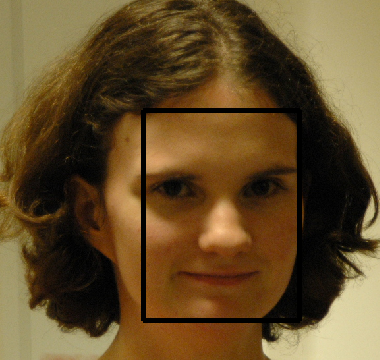
\includegraphics[height=1.2in]{figures_cvpr/promo/case1/detector.png}& \hspace{3mm}
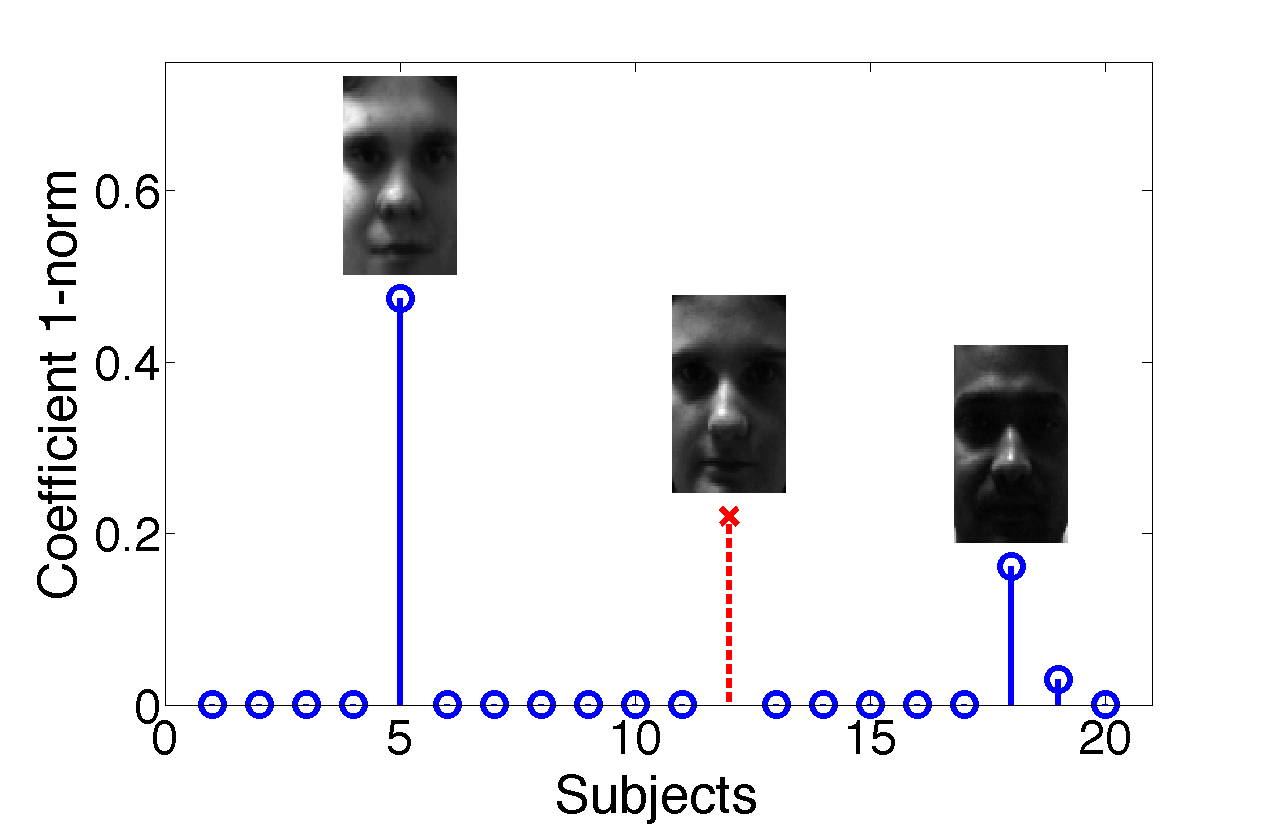
\includegraphics[height=1.2in]{figures_cvpr/promo/case1/sci_with_axis_face_case1.png} \\
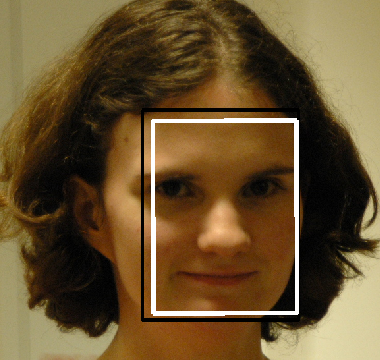
\includegraphics[height=1.2in]{figures_cvpr/promo/alignment_and_detector.png}& \hspace{3mm}
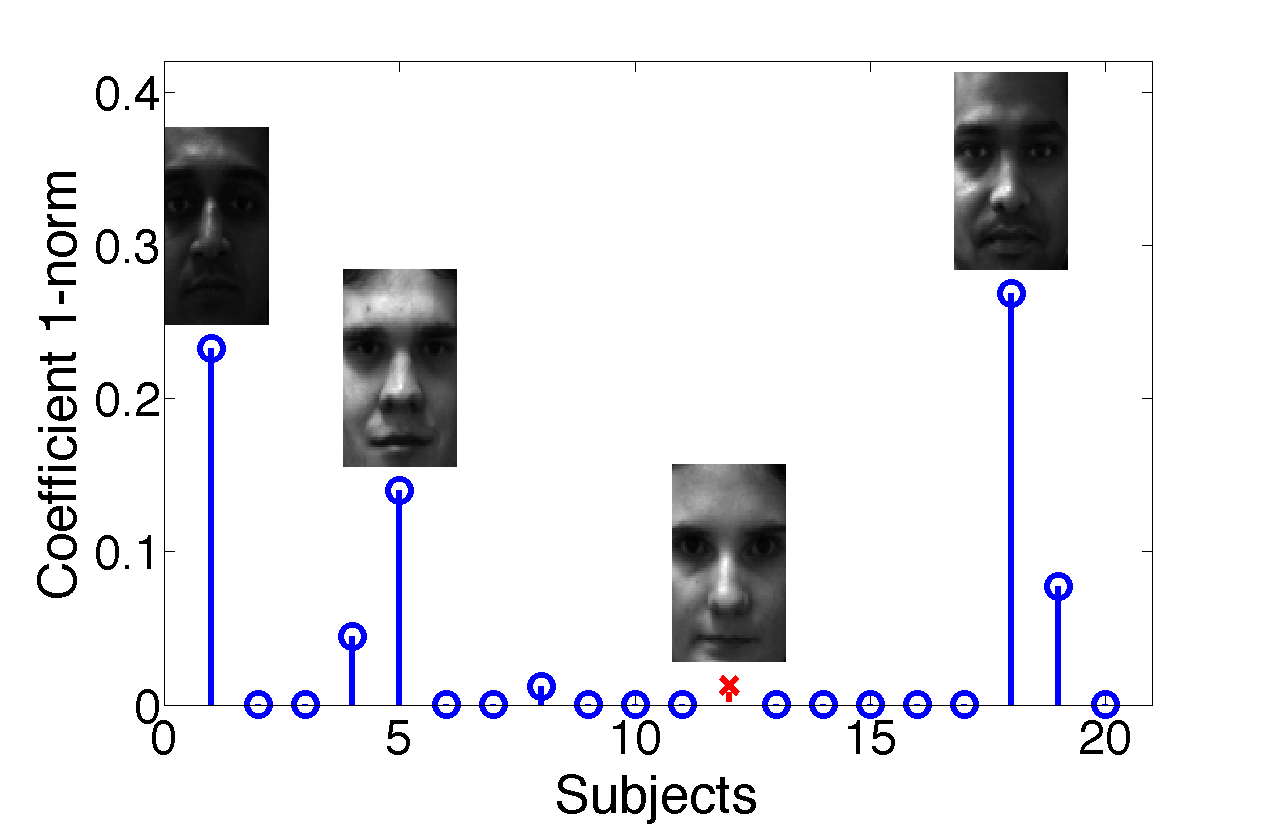
\includegraphics[height=1.2in]{figures_cvpr/promo/case2/sci_with_axis_face_case2.png} \\
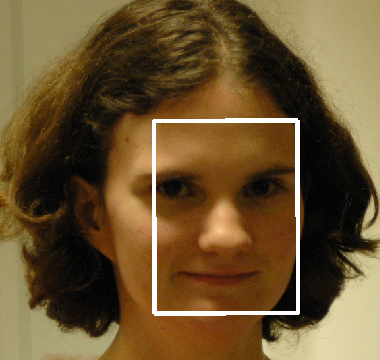
\includegraphics[height=1.2in]{figures_cvpr/promo/case3/alignment.png} & \hspace{3mm}
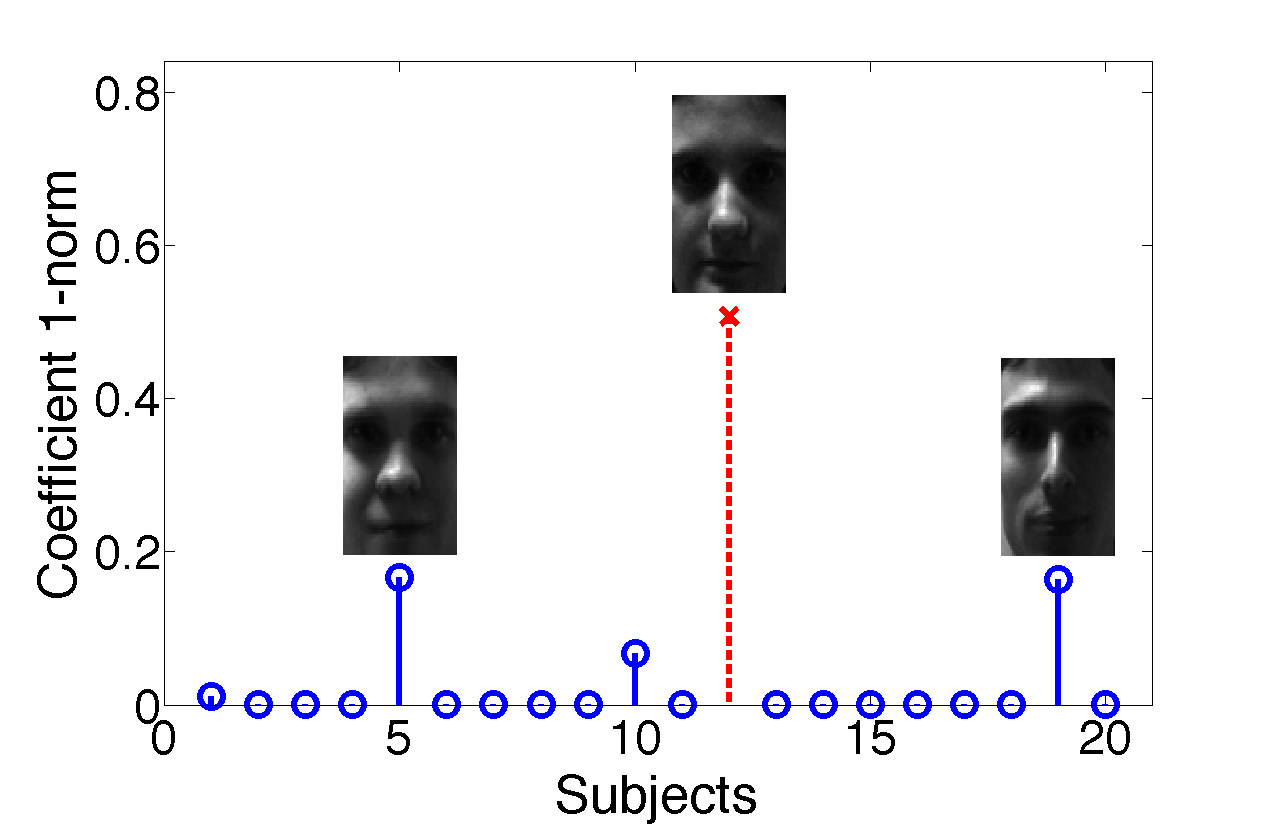
\includegraphics[height=1.2in]{figures_cvpr/promo/case3/sci_with_axis_face_case3.png}
\end{tabular}
\caption{{\bf Compound effect of registration and illumination}. The task is to identify the girl among 20 subjects, by computing the sparse representation of her input face with respect to the entire training set. The absolute sum of the coefficients associated with each subject is plotted on the right. We also show the faces reconstructed with each subject's training images weighted by the associated sparse coefficients. The red line (cross) corresponds to her true identity, subject 12. {\bf Top:} The input face is from Viola and Jones' face detector (the black box) and all 38 illuminations specified in Section \ref{sec:illumination} are used in the training.  {\bf Middle:} The input face is well-aligned (the white box) with the training by our algorithm specified in Section \ref{sec:registration} but only 24 frontal illuminations are used in the training for recognition (see Section \ref{sec:illumination}). {\bf Bottom:} Informative representation obtained by using both well-aligned input face and sufficient (all 38) illuminations in the training. \vspace{0mm}} 
\label{fig:promo}
\end{figure}

While that work achieves impressive results on public datasets taken under controlled laboratory conditions such as Extended Yale B \cite{Georghiades2001-PAMI}, it fails to address two critical aspects of real world face recognition: significant variations in both the {\em image domain} and in the {\em image value}. We illustrate this with an example in  Figure \ref{fig:promo}. The task is to identify the girl among 20 subjects. If the test face image, say obtained from an off-the-shelf face detector, has even a small amount of registration error against the training images (caused by mild pose, scale, or misalignment), the representation is no longer informative, even if sufficient illuminations are present in the training as shown in Figure \ref{fig:promo} top. In addition, in order to sufficiently interpolate the illumination of a typical indoor (or outdoor) environment, illuminations from behind the subject are also needed in the training. Otherwise, even for perfectly aligned test images, the representation will not necessarily be sparse or informative, as shown by the example in Figure \ref{fig:promo} middle. Unfortunately, most public face databases lack images with a significant component of rear (more than 90 degrees from frontal) illumination, either for training or testing.\vspace{0mm}

\paragraph{Contributions.} In this chapter, we show how the two {\em strongly coupled} issues of registration and illumination can be naturally addressed within the sparse representation framework. We show that face registration, a challenging nonlinear problem, can be solved by a series of linear programs that iteratively minimize the sparsity of the registration error. This leads to an efficient and effective alignment algorithm for face images that works for a large range of variation in translation, rotation, scale, and pose, even when the face is only partially visible due to eyeglasses, hats, closed eyes and open mouth, sensor saturation, etc.  We also propose a sufficient, if not the smallest, set of training illuminations that is capable of interpolating typical indoor and outdoor lighting, along with a practical hardware system for capturing them.  Finally, we demonstrate the effectiveness of the proposed new methods with a complete face recognition system that is {\em simple, stable, and scalable}. 
The proposed algorithm performs robust automatic recognition of subjects from loosely controlled images taken both indoors and outdoors, using labeled frontal views of the subjects' faces under the proposed illuminations for training and an off-the-shelf face detector\footnote{In this chapter, we use the OpenCV implementation of the Viola and Jones' face detector \cite{Viola2004-IJCV}.} to detect faces in images. \vspace{0mm}

\section{Handling Practical Registration Error}\label{sec:registration}\vspace{0mm}
As demonstrated in Figure \ref{fig:promo} top, the main limitation of the {\em sparse representation and classification} (SRC) algorithm of \cite{Wright2009-PAMI} is the assumption of pixel-accurate alignment between the test image and the training set. This leads to brittleness under pose and misalignment, making it inappropriate for deployment outside a laboratory setting. In this section, we show how this weakness can be rectified while still preserving the conceptual simplicity and good recognition performance of SRC. 

SRC assumes access to a database of multiple registered training images per subject, taken under varying illuminations. The images of subject $i$, stacked as vectors, form a matrix $A_i \in \Re^{m \times n_i}$. Taken together, all of the images form a large matrix $A = [ A_1 \mid A_2 \mid \dots \mid A_K ] \in \Re^{m \times n}$. As argued in \cite{Wright2009-PAMI}, a well-aligned test image $\y_0$ can be represented as a sparse linear combination $A \x_0$ of all of the images in the database,\footnote{We assume the illuminations in the training set are sufficient. We will address how to ensure illumination sufficiency in the next section.} plus a sparse error $\e_0$ due to occlusion. The sparse representation can be recovered by minimizing the sum or the 1-norm\footnote{The 1-norm of a vector $\x$ is the sum of absolute values of the entries.} of $\x$ and $\e$:\vspace{0mm}

\begin{equation}
\min \| \x \|_1 + \| \e\|_1 \quad \subj \quad \y_0 = A \x + \e.
\label{eqn:robust-l1}\vspace{0mm}
\end{equation}
Now suppose that $\y_0$ is subject to some pose or misalignment, so that instead of observing $\y_0$, we observe the warped image $\y = \y_0 \circ \tau^{-1}$, for some transformation $\tau \in T$ where $T$ is a finite-dimensional group of transformations acting on the image domain.  The transformed image $\y$ no longer has a sparse representation of the form $\y = A \x_0 + \e_0$, and naively applying the algorithm of \cite{Wright2009-PAMI} is no longer appropriate, as seen in Figure \ref{fig:promo} top. \vspace{0mm}

\paragraph{Batch and individual alignment.} Notice that if the true deformation $\tau^{-1}$ can be found, then we can apply its inverse $\tau$ to the test image and it again becomes possible to find a sparse representation of the resulting image, as $\y \circ \tau = A \x_0 + \e_0$.  This sparsity provides a strong cue for finding the correct deformation $\tau$: conceptually, one would like to seek a transformation $\tau$ that allows the sparsest representation, by solving\vspace{0mm}
\begin{equation} \label{eqn:L1-L1-conceptual}
\hat{\tau} = \arg\hspace{-2.5mm}\min_{\x,\e,\tau \in T} \| \x \|_1 + \| \e \|_1 \quad \subj \quad \y \circ \tau = A \x + \e. \vspace{0mm}
\end{equation}
For fixed $\tau$, this problem is jointly convex in $\x$ and $\e$. However, as a simultaneous optimization over the coefficients $\x$, error representation $\e$, and transformation $\tau$, it is a difficult, nonconvex optimization problem. One source of difficulty is the presence of multiple faces in the matrix $A$: \eqref{eqn:L1-L1-conceptual} has many local minima that correspond to aligning $\y$ to different subjects. In this sense, the misaligned recognition problem differs from the well-aligned version studied in \cite{Wright2009-PAMI}. For the well-aligned case, it is possible to directly solve for a global representation, with no concern for local minima. With possible misalignment, it is more appropriate to seek the best alignment of the test face with each subject $i$:\vspace{0mm}
\begin{equation} \label{eqn:per-subject-L1}
\hat \tau_i = \arg\hspace{-2.5mm}\min_{\x,\e,\tau_i \in T} \| \e \|_1 \quad \subj \quad \y \circ \tau_i = A_i \x + \e.\vspace{0mm}
\end{equation}
We no longer penalize $\| \x \|_1$, since $A_i$ consists of only images of subject $i$ and so $\x$ is no longer expected to be sparse.\vspace{0mm}

\paragraph{Alignment via iterative $\ell^1$-minimization.} While the problem \eqref{eqn:per-subject-L1} is still nonconvex, for cases of practical interest in face recognition, a good initial guess for the transformation is available, e.g., from the output of a face detector. We can refine this initialization to an estimate of the true transformation by repeatedly linearizing about  the current estimate of $\tau$, and seeking representations of the form:\vspace{0mm}
\begin{equation}
\y\circ \tau + J \Delta \tau = A_i \x + \e.\vspace{0mm}
\end{equation}
Here, $J = \frac{\partial}{\partial \tau} \y \circ \tau$ is the Jacobian of $\y \circ \tau$ with respect to the transformation parameters $\tau$, and $\Delta \tau$ is the step in $\tau$. The above equation is underdetermined if we allow the registration error $\e$ to be arbitrary. Near the correct alignment we expect the aligned testing image to differ from $A_i \x$ only for the minority of the pixels corrupted by occlusions. Thus, we seek a deformation step $\Delta \tau$ that best sparsifies of the registration error $\e$, in terms of its $\ell^1$-norm: \vspace{0mm}
\begin{equation}
\Delta\hat{\tau}_1 = \arg\hspace{-3.5mm}\min_{\x,\e,\Delta\tau \in T} \| \e \|_1 \quad \subj \quad \y + J \Delta \tau = A_i \x + \e.\vspace{0mm}
\label{eqn:L1-align}
\end{equation}
Notice that this is different from the popular choice that minimizes the 2-norm of the registration error:\vspace{0mm}
\begin{equation}
\Delta\hat{\tau}_2 = \arg\hspace{-3.5mm}\min_{\x,\e,\Delta\tau \in T} \| \e \|_2 \quad \subj \quad \y + J \Delta \tau = A_i \x + \e,\vspace{0mm}
\label{eqn:L2-align}
\end{equation}
which is also equivalent to finding the deformation step $\Delta  \tau$ by solving the least-square problem: $\min \|\y + J\Delta \tau - A_i \x \|_2$. Empirically, we find that if there is only small noise between $\y_0$ and $A_i\x$, both \eqref{eqn:L1-align} and $\eqref{eqn:L2-align}$ have similar performance.  However, if there are occlusions in $\y_0$, iterative $\ell^1$-minimization \eqref{eqn:L1-align} is significantly better than iterative $\ell^2$-minimization \eqref{eqn:L2-align}. Figure \ref{fig:L1-L2-align} shows an example.
\begin{figure}
\centering
\begin{tabular}{cccc}
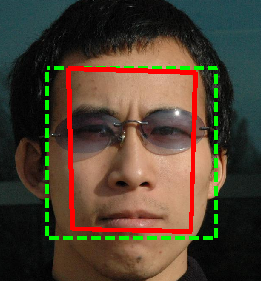
\includegraphics[height=1.2in]{figures_cvpr/L1_cropped} &

\includegraphics[height=1.2in]{figures_cvpr/y_warp_L1} &
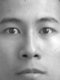
\includegraphics[height=1.2in]{figures_cvpr/y_hat_L1} &
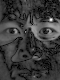
\includegraphics[height=1.2in]{figures_cvpr/e_L1} \\
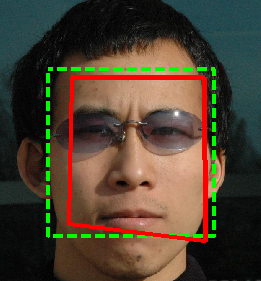
\includegraphics[height=1.2in]{figures_cvpr/L2_cropped} &
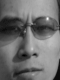
\includegraphics[height=1.2in]{figures_cvpr/y_warp_L2} &
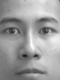
\includegraphics[height=1.2in]{figures_cvpr/y_hat_L2} &
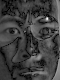
\includegraphics[height=1.2in]{figures_cvpr/e_L2} \\
(a) & (b) & (c) & (d)
\end{tabular}
\caption{{\bf Comparing alignment of a subject wearing sunglasses by 
$\ell^1$ and $\ell^2$ minimization.} 
{\bf Top:} alignment result of minimizing $\|\e\|_1$; {\bf Bottom:} 
result of minimizing $\|\e\|_2$. (a) {\em Green (dotted):} Initial face boundary
given by the face detector, {\em Red (solid):} Alignment result shown on the same
face; (b) warped testing image using the estimated transformation $\y_0$; 
(c) reconstructed face $A_i\x$ using the training; (d) image of error $\e$. \vspace{0mm}}\label{fig:L1-L2-align}
\vspace{0mm}\end{figure}

In addition to normalizing the training images (which is done once), it is important to normalize the warped testing image $\y \circ \tau$ as the algorithm runs.  Without normalization, the algorithm may fall into a degenerate global minimum corresponding to expanding a single black pixel in the test image.  Normalization is done by replacing the linearization of $\y \circ \tau$ with a linearization of the normalized version $\tilde \y(\tau) = \frac{\y \circ \tau}{\|\y \circ \tau\|_2}$.  The proposed alignment algorithm can be easily extended to work in a {\em multiscale} fashion, with benefits both in convergence behavior and computational cost.  The alignment algorithm is simply run to completion on progressively less down-sampled versions of the training and testing images, using the result of one level to initialize the next.  \vspace{0mm}

\paragraph{Robust recognition by sparse representation.}
Once the best transformation $\tau_i$ has been computed for each subject $i$, the training sets $A_i$ can be aligned to $\y$, and a global sparse representation problem of the form \eqref{eqn:robust-l1} can be solved to obtain a discriminative representation in terms of the entire training set. Moreover, the per-subject alignment residuals $\| \e \|_1$ can be used to prune unpromising candidates from the global optimization, leaving a much smaller and more efficiently solvable problem. The complete optimization procedure is summarized as Algorithm \ref{alg:deformable-src}. \vspace{0mm}
\begin{algorithm}[thb]
\begin{small}
\caption{\bf \small  (Deformable Sparse Recovery and Classification for Face Recognition).} \label{alg:deformable-src}
\begin{algorithmic}[1]
\STATE {\bf Input:} Frontal training images $A_1, A_2, \ldots, A_K \in \Re^{m\times n_i}$ for $K$ subjects,  a test image $\y\in\Re^m$ and a deformation group $T$ considered.
\STATE {\bf for} each subject $k$, 
\STATE \hspace{3mm} $\tau^{(0)} \leftarrow I$.
\STATE \hspace{3mm} {\bf do}
\STATE \hspace{6mm} $\tilde \y(\tau) \leftarrow \frac{\y \circ \tau}{\|\y \circ \tau\|_2}$; \;\;\; $J \leftarrow  \frac{\partial}{\partial \tau} \tilde\y(\tau)  \bigr|_{\tau^{(i)}} $;\vspace{0mm}
%\STATE \hspace{6mm} $(\hat \x, \hat \e, \Delta \tau) \leftarrow \left\{\begin{array}{l} \arg \min_{\x,\e,\Delta \tau} \| \e \|_1 \\  \subj \; \y + J \Delta \tau = A_k \x + \e \end{array}\right.$
\STATE \hspace{6mm} $ \Delta \tau =  \arg\min \; \| \e \|_1  \; \mathrm{s.t.} \; \tilde \y + J \Delta \tau = A_k \x + \e, \; \x \ge \0.$
\STATE \hspace{6mm} $\tau^{(i+1)} \leftarrow \tau^{(i)} + \Delta \tau$; 
\STATE \hspace{3mm} {\bf while} $\| \tau^{(i+1)} - \tau^{(i)} \| \ge \varepsilon$.
\STATE {\bf end}
\STATE Keep the top $S$ candidates $k_1, \ldots, k_S$ with the smallest residuals $\|\e\|_1$. 
\STATE Set $A \leftarrow \big[ A_{k_1} \circ \tau_{k_1}^{-1} \mid A_{k_2} \circ \tau_{k_2}^{-1} \mid \dots \mid A_{k_S} \circ \tau_{k_S}^{-1} \big]$. 
\STATE Solve the $\ell^1$-minimization problem: \vspace{0mm}
$$\hat{\x} = \arg \min_{\x, \e} \| \x \|_1 + \|\e\|_1 \;\; \text{subj} \;\; \y = A \x + \e, \;\x \ge 0.\vspace{0mm}$$
\STATE Compute residuals $r_i(\y) = \| {\y} - {A}_i \, \hat{\x}_i \|_2$ for $i = k_1, \dots, k_S$.
\STATE {\bf Output:} $\mbox{identity}(\y) = \arg\min_i r_i(\y)$.
\end{algorithmic}
\end{small}
\end{algorithm}\vspace{0mm}

The most important free parameter in Algorithm \ref{alg:deformable-src} is the class of deformations $T$. In our experiments, we typically use 2D similarity transformations, $T = \mathbb{SE}(2)\times \Re_+$, for compensating error incurred by face detector, or 2D projective transformations, $T = \mathbb{GL}(3)$, for handling some pose variation. The parameter $S$ decides how many top candidates get considered together to provide a sparse representation for the test image. If $S = 1$, the algorithm reduces to classification by registration error; but considering the test image might be an invalid subject, we typically choose $S = 10$. Since valid images have a sparse representation in terms of this larger set, we can reject invalid test images using the {\em sparsity concentration index} proposed in \cite{Wright2009-PAMI}. We have implemented a fast linear program for our algorithm in C. Running on a 2.8GHz Mac Pro, alignment takes 0.65 second per subject for our database. \vspace{0mm}


\paragraph{Simulations and experiments on region of attraction.} We now perform simulations and experiments demonstrating the effectiveness of the individual alignment procedure outlined in the previous section, and clarifying its operating range. We delay large-scale recognition experiments to Section \ref{sec:experiment}, after we have discussed the issue of illumination in the next section.\vspace{0mm}
\begin{enumerate}	
\item{\em 2D Deformation.}  We first verify the effectiveness of our alignment algorithm with images from the CMU Multi-PIE Database \cite{Gross2008-FGR}. We select 120 subjects in Session 2, use 11 illuminations per person from Session 2 for training, and test on one new illumination from Session 3.\footnote{The training are illuminations $\{0, 1,3,5,7,9,11,13,14,16,18\}$ of \cite{Gross2008-FGR}, and the testing is the illumination 10. } We manually select eye corners in both training and testing as the ground truth for registration. We down-sample the images to $80\times 60$ pixels\footnote{Unless otherwise stated, this will be the default resolution at which we prepare all our training and testing datasets and run all our experiments.} and the distance between the two outer eye corners are normalized to be 50 pixels for each person. We introduce artificial deformation to the testing image with a combination of translation or rotation. We consider a registration successful if the difference between the final registration error is within 1\% of the error by manual registration.  Figure \ref{fig:attraction} shows the percentage of successful registrations for the 120 subjects for each artificial deformation. The results suggest that our algorithm works extremely well with translation up to 20\% of the eye distance (or 10 pixels) in all directions and up to $30^\circ$ in-plane rotation. We have also tested our alignment algorithm with scale variation and it can handle up to 25\% change in scale.

We have gathered the statistics of the Viola and Jones' face detector on the Multi-PIE datasets. For 4,600 frontal images of 230 subjects under 20 different illuminations, using manual registration as the ground truth, the average misalignment error of the detected faces is about 6 pixels and the variation in scale is 17\%. This falls safely inside the range of attraction for our alignment algorithm.
\begin{figure}
\centering
\begin{tabular}{cc}
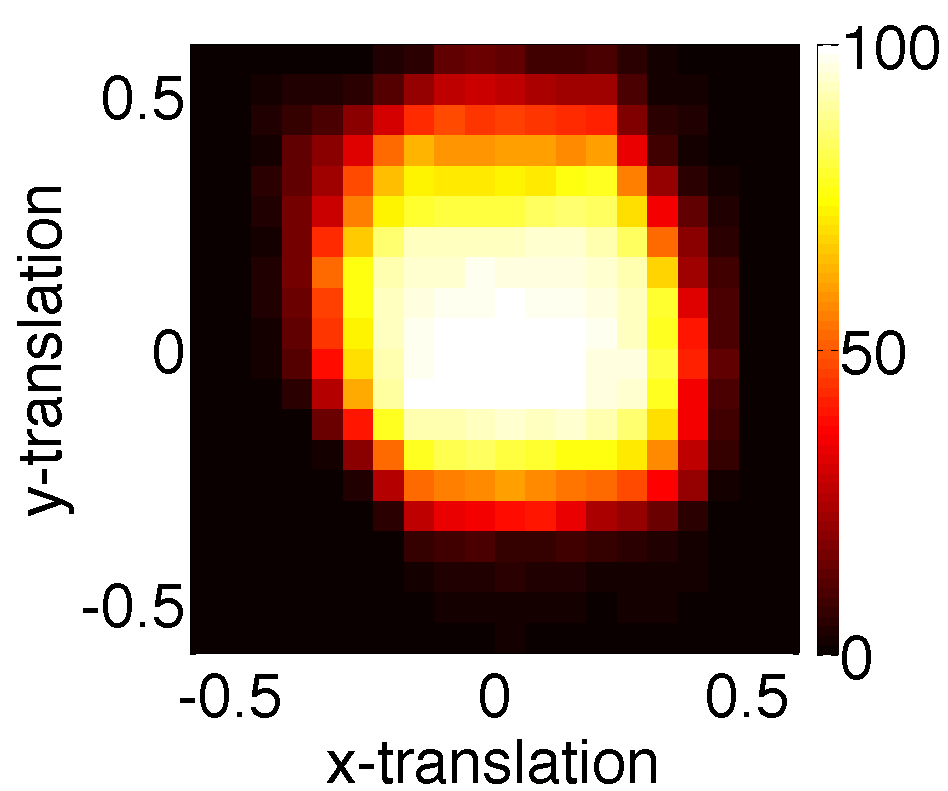
\includegraphics[height=1.8in]{figures_cvpr/translation_fig3.png} &
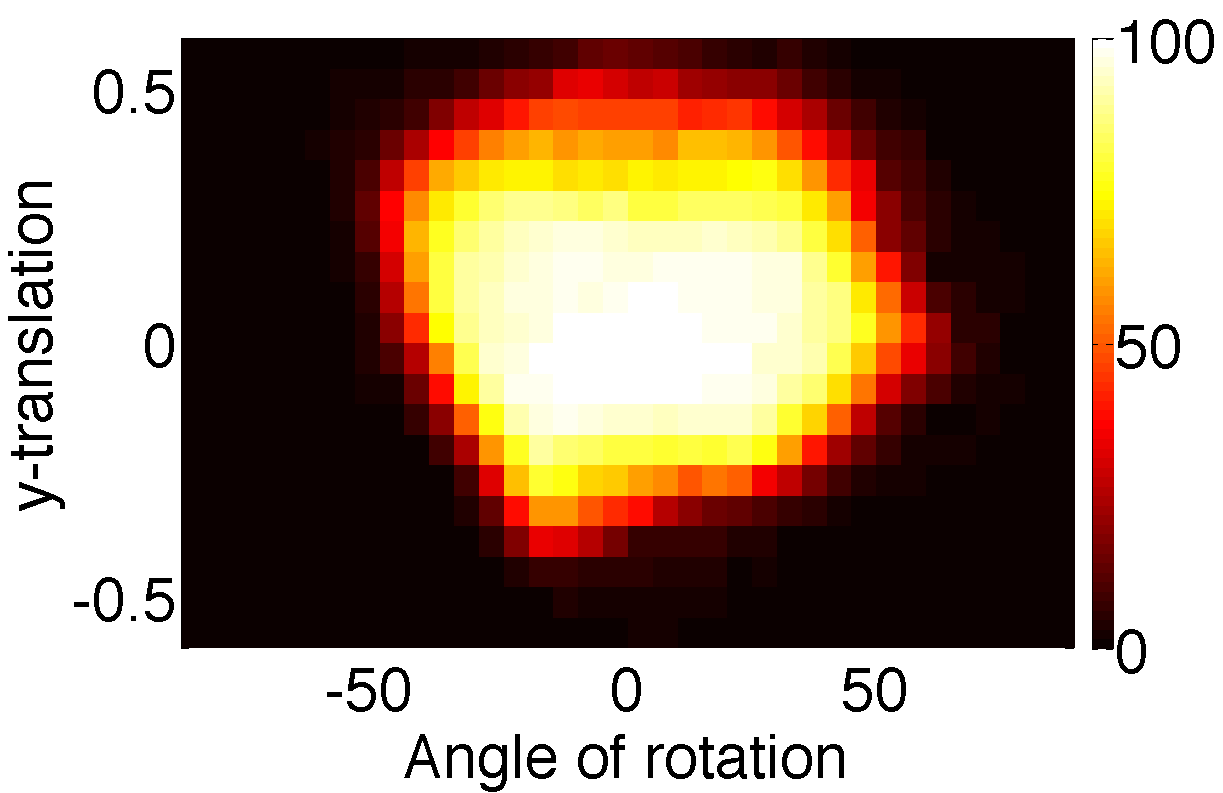
\includegraphics[height=1.9in]{figures_cvpr/translation_rotation_fig1.png}\\
(a)&(b)
\end{tabular}
\vspace{0mm}
\caption{{\bf Region of attraction.} Fraction of subjects for which the algorithm successfully aligns a synthetically perturbed test image.  The amount of translation is expressed as a fraction of the distance between the outer eye corners, and the amount of in-plane rotation in degrees. {\bf Left:} Simultaneous translation in $x$ and $y$ directions. More than $90\%$ of the subjects were correctly aligned for any combination of $x$ and $y$ translations, each upto $0.2$. {\bf Right:} Simultaneous translation in $y$ direction and in-plane rotation $\theta$. More than 90\% of the subjects were correctly aligned for any combination of $y$ translation upto $0.2$ and $\theta$ upto $25^\circ$.}
\label{fig:attraction}
\end{figure}

\vspace{0mm}
\item{\em 3D Pose Variation.} As densely sampled pose and illumination face images are not available in any of the public databases, including Multi-PIE, we have collected our own dataset using our own system (to be introduced in the next section.) We use frontal face images of a subject under the 38 illuminations proposed in the next section as training. For testing, we collect the image of the subject under a typical indoor lighting condition at pose ranging from $-90^\circ$ to $+90^\circ$ with step size 5.625$^\circ$, a total of 33 poses. We use Viola and Jones' face detector to initialize our alignment algorithm. 
%whenever it succeeds. For extreme poses where the detector fails (usually for poses $> 45^\circ$), we use manual initialization by putting a reasonable square window around the face. 
Figure \ref{fig:pose-alignment} shows the typical alignment results of our algorithm, working surprisingly well with poses up to $\pm 45^\circ$. \vspace{0mm}
\begin{figure}
\centering
\begin{tabular}{ccccc}

\includegraphics[height=1in]{figures_cvpr/5} &
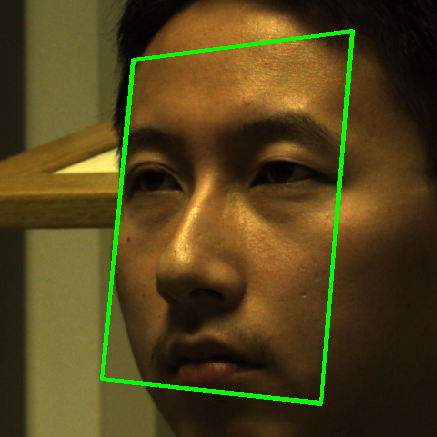
\includegraphics[height=1in]{figures_cvpr/7} &
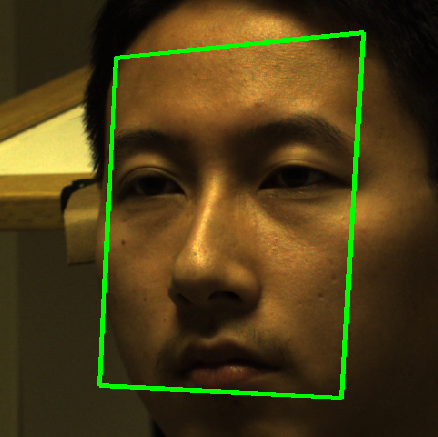
\includegraphics[height=1in]{figures_cvpr/09} &
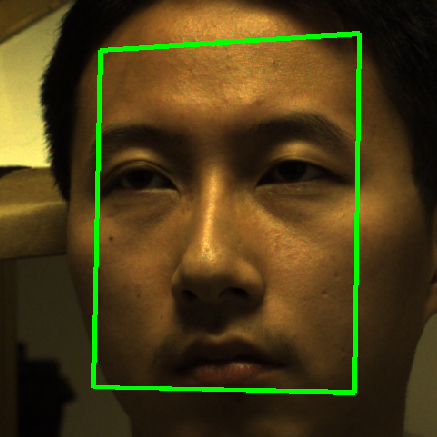
\includegraphics[height=1in]{figures_cvpr/11} &
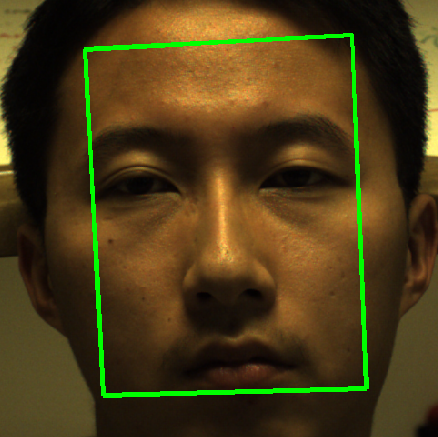
\includegraphics[height=1in]{figures_cvpr/13} \\
(a) & (b) & (c) & (d) & (e)\vspace{3mm}\\
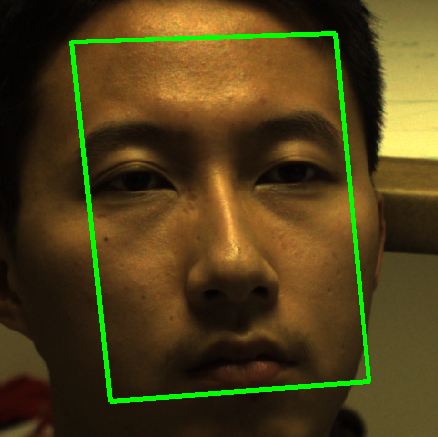
\includegraphics[height=1in]{figures_cvpr/15} &

\includegraphics[height=1in]{figures_cvpr/17} &
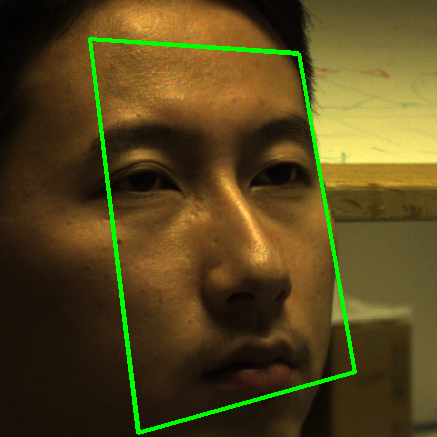
\includegraphics[height=1in]{figures_cvpr/19} &
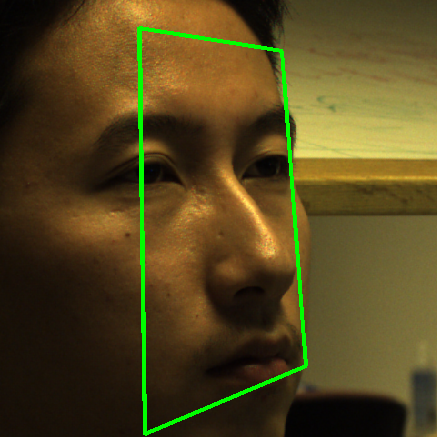
\includegraphics[height=1in]{figures_cvpr/21} &

\includegraphics[height=1in]{figures_cvpr/3} \\
(f) & (g) & (h) & (i) & (j)
\end{tabular}
\caption{{\bf Aligning different poses to frontal training images.} {\bf (a) to (i):}  good alignment for pose from $-45^{\circ}$
to $+45^{\circ}$. {\bf (j):} a case when the algorithm fails for an extreme pose ($>45^{\circ}$).\vspace{0mm}
}\label{fig:pose-alignment}
\end{figure}
\end{enumerate}

\paragraph{Relationship to existing work.} 
Our modification to SRC roots solidly in the tradition of adding deformation-robustness to face recognition algorithms \cite{Cootes2001-PAMI,Gross2006-PAMI,Wiskott1997-PAMI}. However, the only previous work to investigate face alignment in the context of sparse signal representation and SRC is the work of \cite{Huang2008-CVPR}. They consider the case where the training images themselves are misaligned and allow one deformation per training image. They linearize the training rather than the test, which is computationally more costly as it effectively triples the size of the training set. In addition, as they align the test image to all subjects simultaneously, it potentially is more prone to local minima when the number of subjects increases, as we will see in the following experimental comparisons. \vspace{0mm}
\begin{enumerate}
\item {\em Extended Yale B.} In this experiment, we have used the exact experimental settings in \cite{Huang2008-CVPR}. 
20 subjects are selected and each has 32 frontal images (selected at random) as training and another 32 for testing. An artificial translation
of 10 pixels (in both $x$ and $y$ directions) is introduced to the test. For our algorithm we down-sample all the images
to $88\times 80$ for memory reasons, whereas the work of \cite{Huang2008-CVPR} uses random projections. Our algorithm achieves the recognition rate 88.59\% which is on par with the result reported in \cite{Huang2008-CVPR}.
However, this special setting is disadvantageous to our algorithm: The use of cropped test images introduces boundary effects, and the presence of very extreme illuminations makes enforcing nonnegativity of $\x$ (as in Algorithm 1 less appropriate. We further discuss the justification for nonnegativity in the next section.\vspace{0mm}
\item {\em CMU Multi-PIE.} In this experiment, we choose 160 subjects from the CMU Multi-PIE, 11 training images from Session 2
and 1 test image from Session 3 per person. The setting is exactly the same as the previous experiment on 2D deformation, 
except that we have more subjects. We again 
work with downsampled images of size $80\times 60$. An artificial translation of 5 
pixels (in both $x$ and $y$ directions) was induced in the test image. The algorithm of \cite{Huang2008-CVPR} achieves
a recognition rate of 73.75\%,\footnote{That algorithm has two free parameters - $l$ and $d$. For this experiment we chose 
$l = 1$ and $d = 514$ (higher values may get a better recognition rate at the expense of higher running time).
} while ours does 90.625\%. \end{enumerate}\vspace{0mm}
				
\section{Handling Practical Illumination Variation}\label{sec:illumination}\vspace{0mm}
In the above section, we have made the assumption that the test image, although taken under some arbitrary illumination, can be linearly interpolated by a finite number of training illuminations.  Under what conditions is this a reasonable assumption to make?  What can we say from first principles about how the training images should be chosen?  

\paragraph{The illumination model}
First, let us assume that the illumination if the subject's face is distant.  This model will be a good approximation as long as distance to the nearest light source is much larger than the person's face.  If we further assume that the object is convex so that there is no self-shadowing, the illumination incident on a surface patch will depend only on its orientation, and not on its position.  Furthermore, if the object is lambertian, the intensity of the image of a given patch of object will not depend on its position either.  Since each pixel in the image corresponds to some patch on the object, the vector of image intensities is a linear function of the radiance of the corresponding portions of the object.  Consider the vector space of all illuminations of the object.  These are just positive functions (or more generally, distributions) defined on the sphere, where each point on the sphere corresponds to a direction of incoming light.  Consider the vector space formed by the light exiting the object.  This too is a positive function defined on the sphere, where now each point on the sphere corresponds to the normal of a patch on the object (or any other patch with the same normal).  Under the Lambertian assumption, the radiance of a patch depends on the cosine of the incident angle of incoming light, and is integrated over the half-sphere of illumination that the patch can "see".
Thus, the surface of the object acts on the sphere in a manner very similar to a half-cosine approximation to a low-pass filter for a one-dimensional signal.  Thus the energy leaving the object is disproportionately concentrated in the subspace corresponding to low spatial frequencies.  Since the image is a linear function of this, the space of images of an object will also tend to fall on (the positive portion of) a subspace.   In \cite{Basri2003-PAMI}, Basri showed using spherical harmonic basis functions that nine basis illuminations (corresponding to the lowest frequency spherical harmonics) result in training images that do a good job of linearly interpolating all other training images.  It should be noted, however, that these basis illuminations are not strictly positive, and thus neither are the training images they generate (when rendered on a computer that can handle negative illumination).  \footnote{Note that while the spherical harmonic basis functions have regions where they are negative, this does no necessary preclude this theoretical result from being put to use in practice.  If the geometry of the training illumination system were well calibrated, it would be possible to generate approximations of the positive and (rectified) negative components of the basis illuminations separately, taking the difference of the resulting two images, and storing it using a signed datatype.  Combinations of these images may not be positive, but they may still be good enough to be useful}.

Although a human face is neither perfectly Lambertian nor convex, it has been observed in various empirical studies that one can often get away using a similar number of frontal illuminations to interpolate a wide range of new frontal illuminations that taken under the same laboratory conditions \cite{Georghiades2001-PAMI}. This is the case for many public face datasets, including AR, ORL, PIE, and Multi-PIE.  Unfortunately, we have found that in practice, a training database consisting purely of frontal illuminations is not sufficient to linearly interpolate images of a faces taken under typical indoor or outdoor conditions (see the experiment conducted in Section \ref{sec:own-data}). As illustrated by the example in Figure \ref{fig:promo}, an insufficient number of training illuminations can result in recognition failure. 
To ensure our algorithm works in practice, we need to find a set of training illuminations that are indeed {\em sufficient} to linearly interpolate a wide variety of practical indoor and outdoor illuminations.\vspace{0mm}

\paragraph{Capturing a sufficient set of training illuminations.}   To this end, we have designed a system that can illuminate the subject from all directions above horizontal, while acquiring the subject's frontal images. A sketch of the system is shown in Figure \ref{fig:system}: The illumination system consists of four projectors that display various bright patterns onto the three white walls in the corner of a dark room.  The light reflects off of the walls and illuminates the user's head indirectly.  After taking the frontal illuminations we rotate the chair by 180 degrees and take pictures from the opposite direction.  Having two cameras speeds the process since only the chair needs to be moved in between frontal and rear illuminations.  
Our projector-based system has several advantages over flash-based illumination systems:\vspace{0mm}
\begin{itemize}
\item The illuminations can be defined in software.\vspace{0mm}
\item It is easy to capture many different illuminations.\vspace{0mm}
\item There is no need to mount cameras on walls or construct a large dome.\vspace{0mm}
\item No custom hardware is needed for a basic system.\vspace{0mm}
\end{itemize}
\begin{figure}
\centerline{\hspace{-0.1in}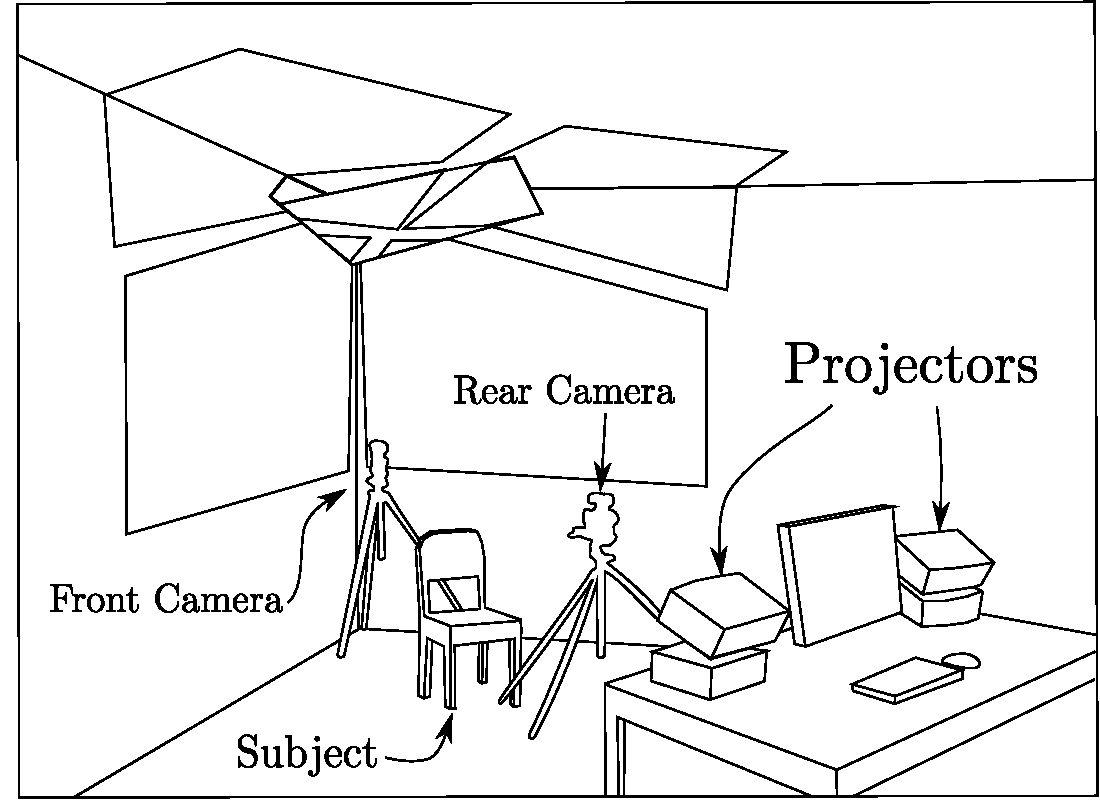
\includegraphics[height=3in]{figures_cvpr/camera_rig.pdf}}
\caption{{\bf Training acquisition system:} Four projectors and two cameras controlled by one computer.\vspace{0mm}}
\label{fig:system}
\end{figure}
With our projector system, our choice of illuminations is constrained only by the need to achieve a good SNR\footnote{Since illuminations with more pixels illuminated will have a better SNR (provided they don't saturate), there is an engineering tradeoff between the SNR and the number of training images we can acquire.}
avoid saturation, and achieve a reasonably short acquisition time.  Two simplifying assumptions that we make is that every pixel is either turned full on or off in every illumination, and that no pixels are shared by illuminations.  Assuming that the pixels are all the way on or all the way off allows us to control the amount of illumination directly with the number of pixels we illuminate, eliminating any influence from gamma curve of the projector. \footnote{Caution; DLP projectors may have very wacky response curves depending on the mode they are in.  Note that controlling the intensity between illuminations is only needed to prevent saturation or low SNR; our algorithm depends on the linearity between the illuminations and the images, not on the relative intensities of the illuminations.} The choice of orthogonal (no pixels in common) illuminations is important; any other non-negative basis illuminations formed from a linear combination of our basis vectors will span a cone of lower volume, and thus the resulting training images might not be able to represent as wide a variety of testing images. 

We ran two experiments to guide our choice of illuminations for our large-scale experiments:\vspace{0mm}  
\begin{itemize}
\item {\em Coverage Experiment.} In the first experiment we attempt to determine what coverage of the sphere is required to achieve good interpolation for test images.  The subject was illuminated by 100 (50 front, 50 back) illuminations arranged in concentric rings centered at the front camera.  Subsets of the training images were chosen, starting at the front camera and adding a ring at a time.  Each time a ring was added to the training illumination set, the average $\ell^1$ registration error (residual) for a set of test images taken under sunlight was computed and plotted in Figure \ref{fig:illumination-patterns} (a).  The more rings of training illuminations are added, the lower the representation error becomes, with diminishing returns.\vspace{0mm}
\item {\em Granularity Experiment.} In the second experiment we attempt to determine how finely divided the illumination sphere should be.  At the first granularity level, the projectors  illuminate the covered area uniformly.  At each subsequent granularity level each illuminated cell is divided in two along its longer side but intensity doubled.  For each granularity level the average $\ell^1$ registration error is computed as in the coverage experiment and shown in Figure \ref{fig:illumination-sufficiency} (b).  Again, diminishing returns are observed as more illuminations are added.\vspace{0mm}  
\end{itemize}
\begin{figure}
\centering
\begin{tabular}{cc}
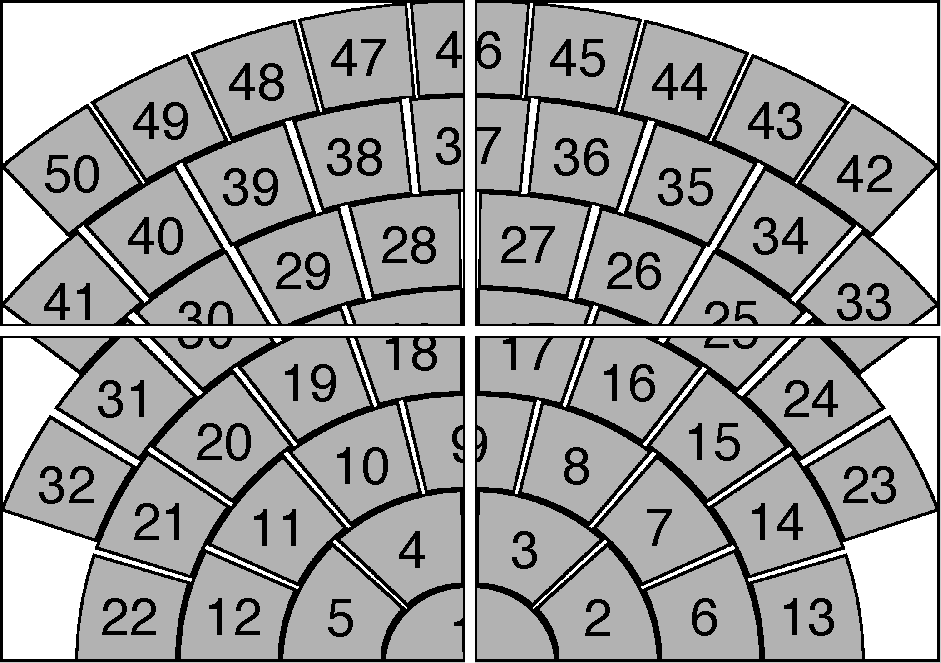
\includegraphics[height=2in]{figures_cvpr/coverage_experiment_asplode.png} &
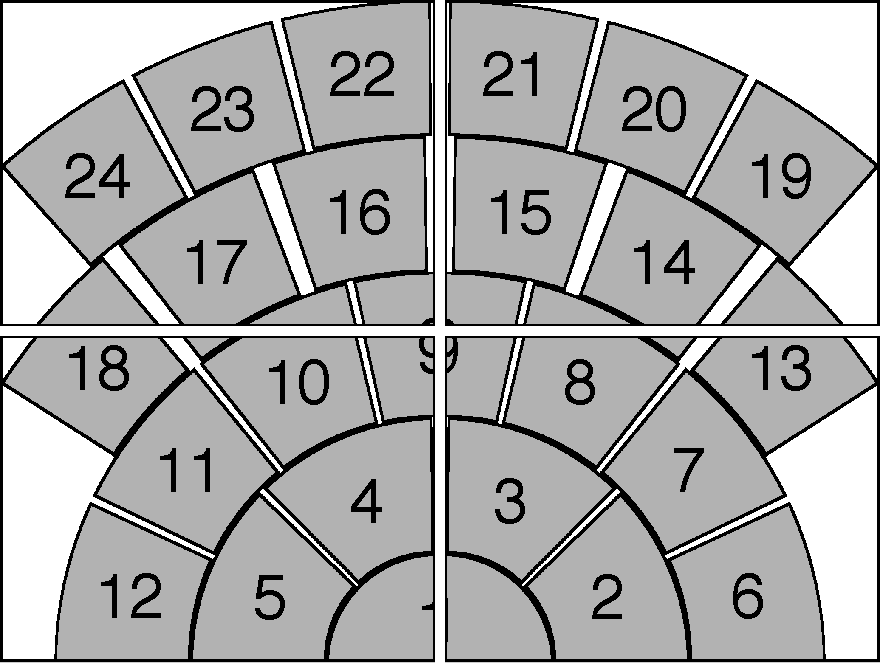
\includegraphics[height=2in]{figures_cvpr/final_cvpr_illuminations_asplode.png} \\
(a) Coverage Experiment & (b) Chosen Illumination Patterns
\end{tabular}\vspace{2mm}
\caption{{\bf Illumination patterns.}   The cells are illuminated in sequence.  For rear illuminations the sequence is reversed.  In the chosen pattern's rear illumination, the cells 1-5 and 7-11 are omitted for a total of 38 illuminations. The four rectangular regions correspond to the four projectors.\vspace{0mm}}
\label{fig:illumination-patterns}
\end{figure}
\begin{figure}
\centering
\begin{tabular}{cc}
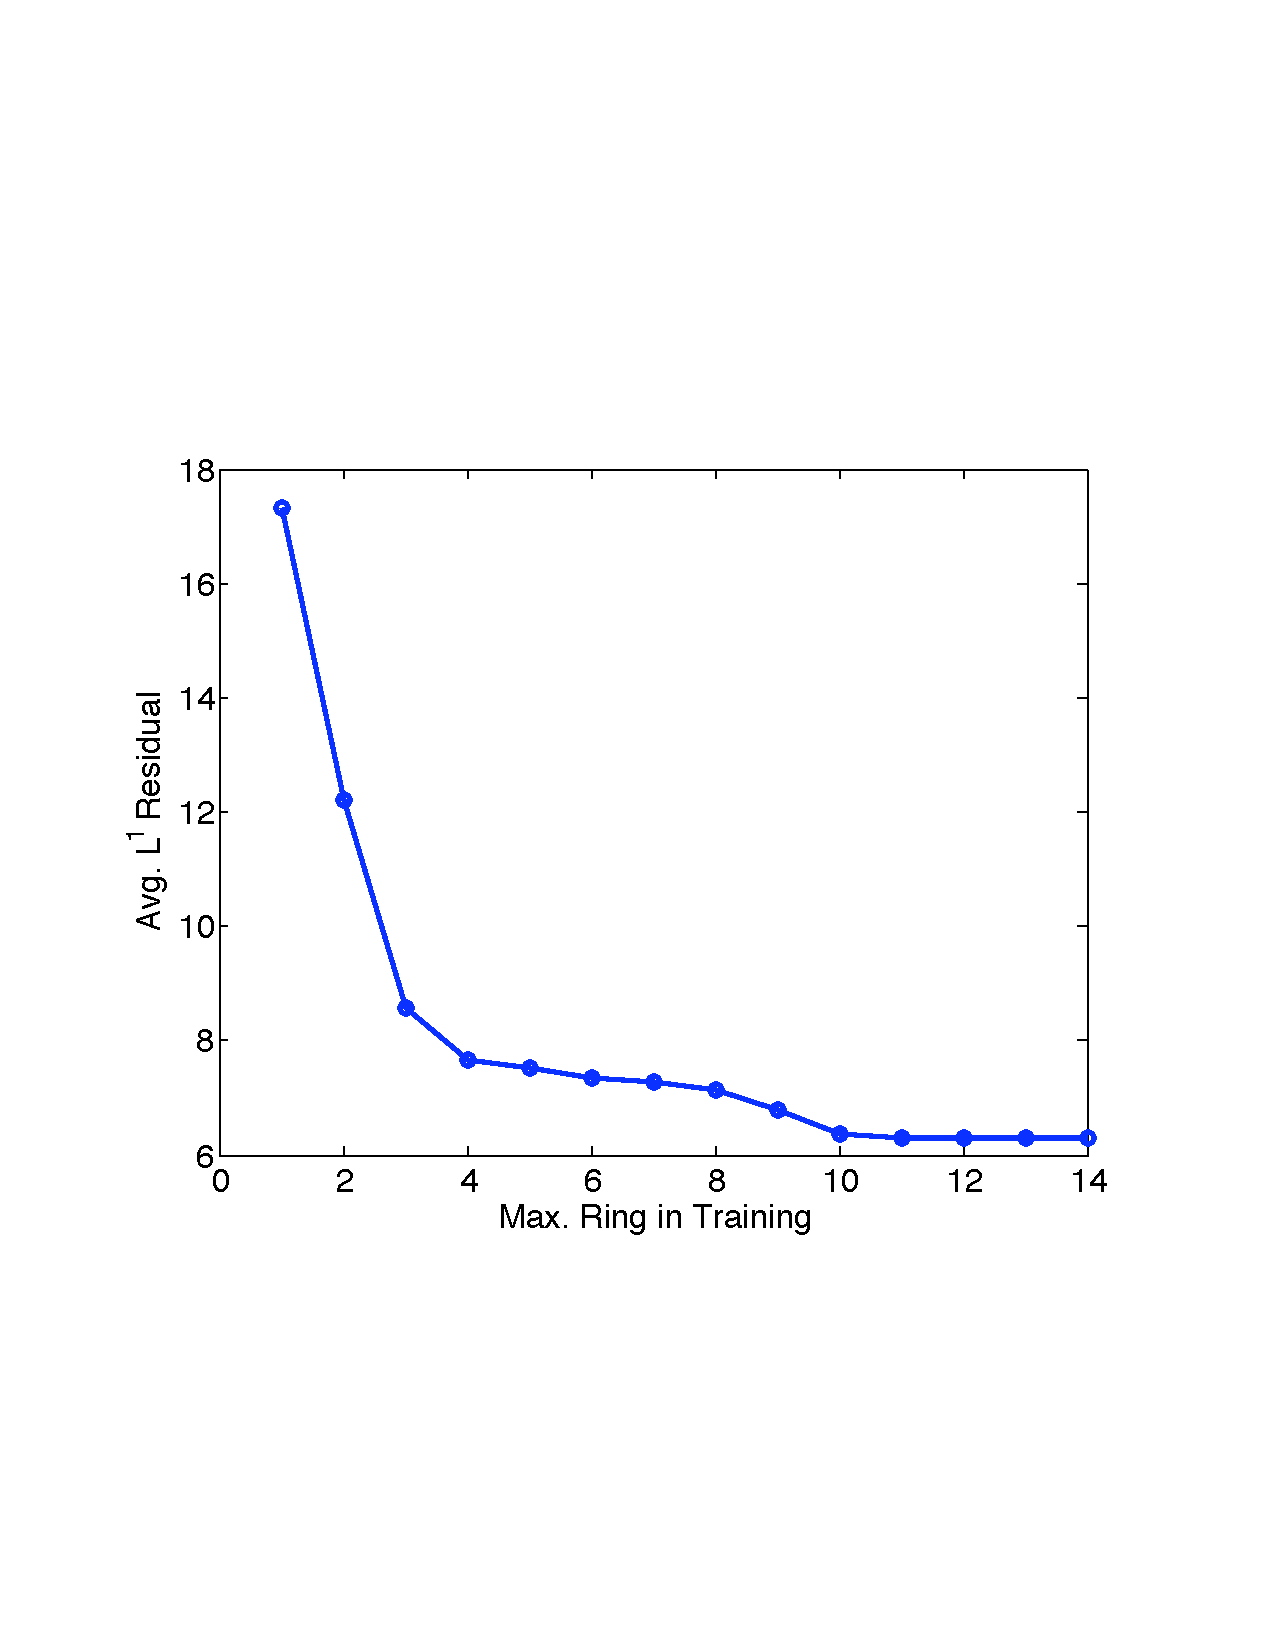
\includegraphics[height=1.5in]{figures_cvpr/illum_results/coverage_sunset.pdf} &
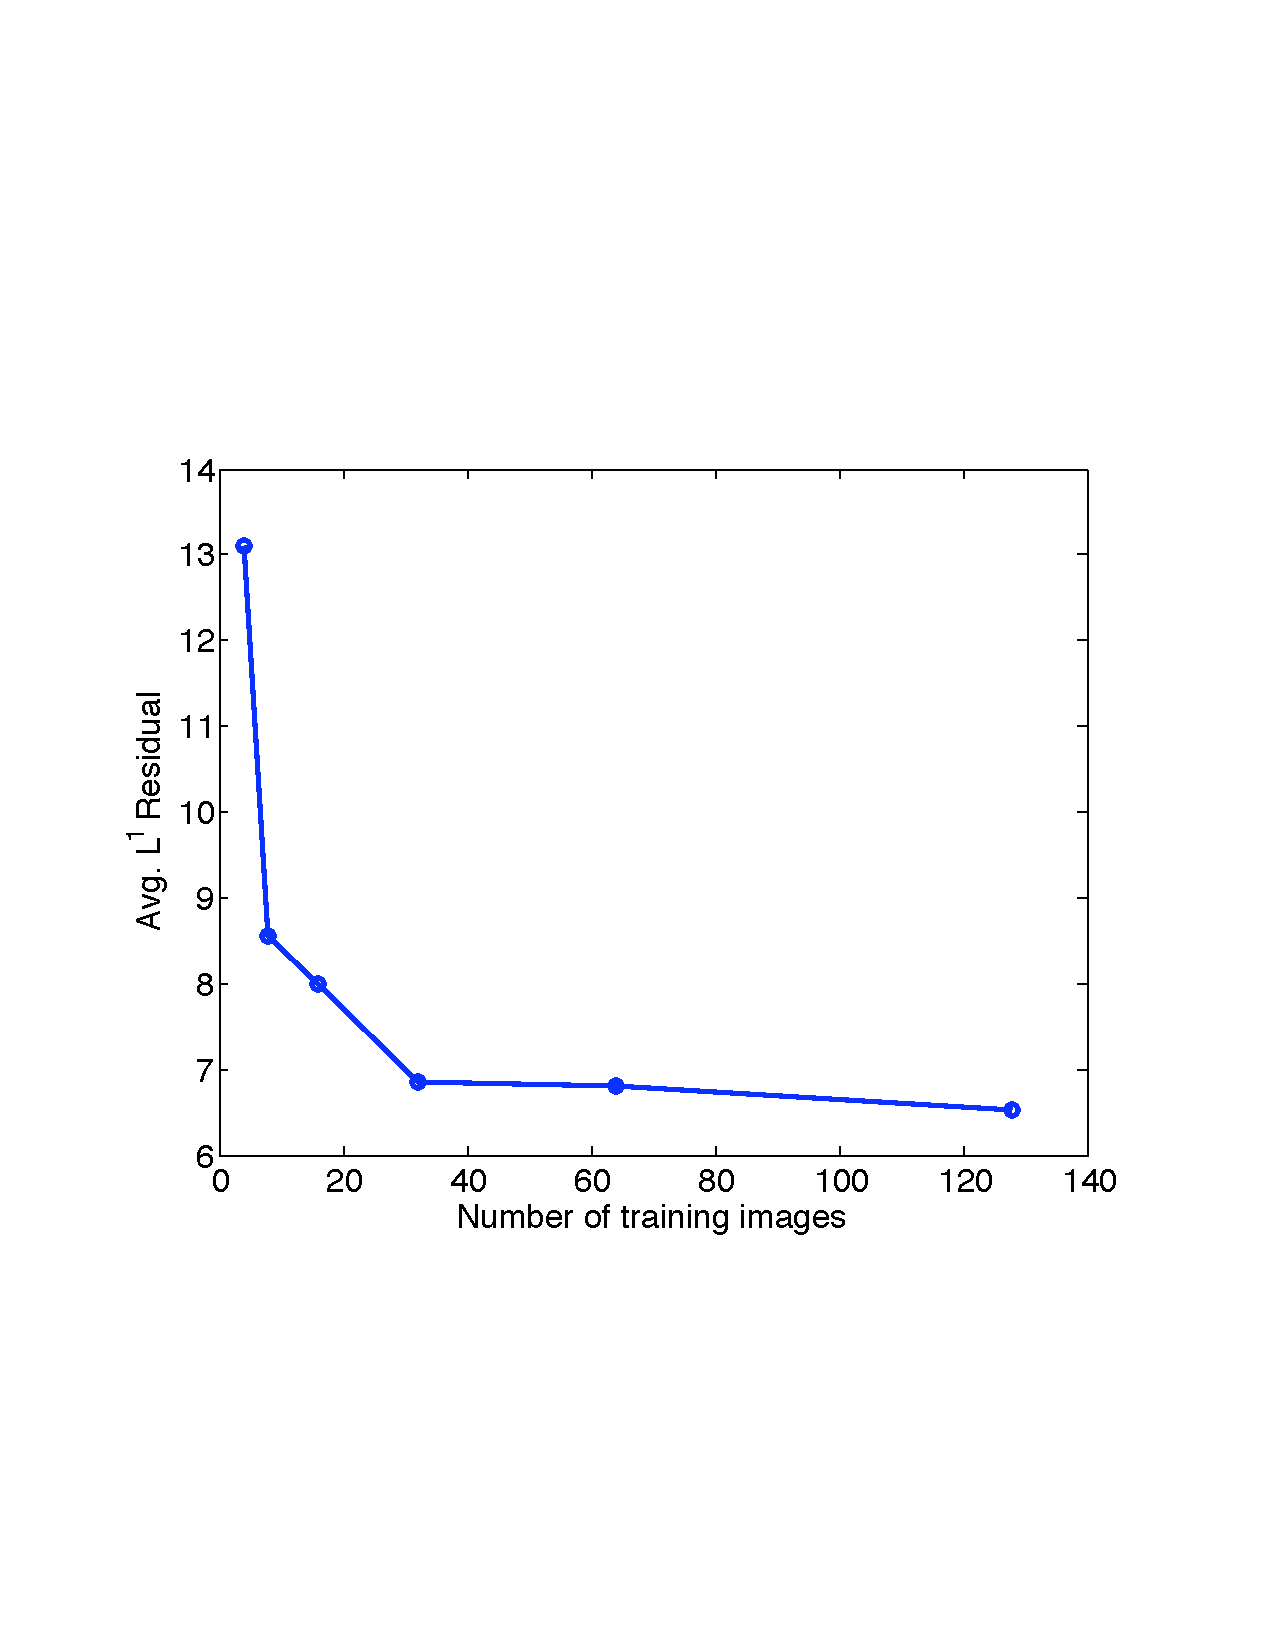
\includegraphics[height=1.5in]{figures_cvpr/illum_results/granularity_sunset.pdf} \\
(a) Coverage & (b) Granularity
\end{tabular}\vspace{2mm}
\caption{{\bf Study of sufficient illuminations.} The average $\ell^1$ registration residual versus different illumination training sets. \vspace{0mm}}
\label{fig:illumination-sufficiency}
\end{figure}

\vspace{0mm}\paragraph{Chosen illumination patterns.} In the plot for the coverage experiment, Figure \ref{fig:illumination-sufficiency} (a), we clearly see two plateau regions: one is after 4 rings and one is after 10 rings. The first four rings represent the typical frontal illuminations, which are present in most public face datasets; however, we see that the residual stabilizes after 10 rings which include some illuminations from the back of the subject. This suggests that although the frontal illuminations can span majority of illumination on the face, some illuminations from the back are needed in the training to emulate the effect of ambient illumination from all directions. In the plot for the granularity experiment, Figure \ref{fig:illumination-sufficiency} (b), we observe that the residual reaches a plateau after four divisions, corresponding to a total of 32 illuminations. Based on the results from both experiments, we decide to partition the area covered by the first 10 rings into a total of 38 cells, whose layout is explained in Figure \ref{fig:illumination-patterns} (b). For our large-scale experiments, we have collected those illuminations for all our subjects.\footnote{It is very likely that with more careful experiments, we can further reduce the number of illuminations needed. Especially some of the frontal illuminations might be redundant. But we keep those in our training anyway as the additional images do not add too much cost to our alignment and recognition algorithm.} 

See below for the 38 images for one subject:
\begin{figure}[h]
\centering
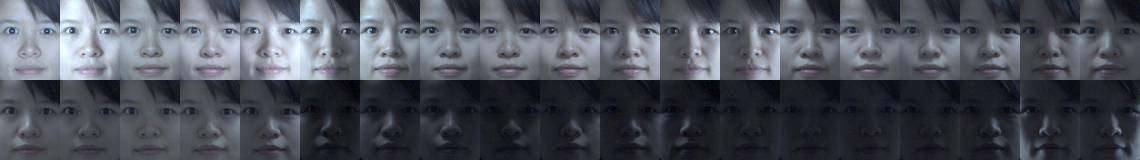
\includegraphics[width=6.3in]{figures_cvpr/training.png}
\end{figure}
\vspace{0mm}

\paragraph{Should Positivity in the Representation Coefficients be Enforced?}
One critical issue in linear illumination models is whether to enforce nonnegativity in the coefficients $\x$, i.e. whether to model illumination using a cone or a subspace.   Some authors, i.e. \cite{Basri2003-PAMI}, have chosen to allow negative components in the coefficient vector $\x$ when representing one image as a sum of other images, and only enforce that the linear combination $A\x$ be positive everywhere.  Unfortunately, for non-convex objects such as faces, enforcing non-negativity of the representation is not sufficient to guarantee that the resulting image of the object is physical.  For example, consider a Lambertian planar object with a cylindrical hole drilled in it that is aligned with the optical axis of an orthographic camera.  Consider two images: one under illumination from a distant point source aligned with the hole, and one off of the hole axis.  Positively weighting the on-axis image and negatively weighting the on-axis image can result in an image where the bottom of the hole is more strongly illuminated than the surrounding plane.  The image is positive, but it is clearly non-physical.  It is worth emphasizing that this phenomenon is a result of some points on an object seeing a restricted subset of the illumination sphere (a violation of convexity),  and not a result of the directionality of the light chosen in the thought experiment.  While the number of coefficients that actually end up negative after optimization is usually very small, we have observed pathological cases where the shadows next to the user's nose in the reconstructed image invert in value.  

Instead of using a smaller set of training images, allowing the coefficients to go negative to try to represent more test illuminations, and risking over-fitting, we decided to enforce non-negativity of the coefficients.  Nonnegative combinations of images are guaranteed to correspond to physically plausible images.  all physical illuminations unless the training images actually span the boundary of the illumination cone. 
Because we have a flexible acquisition system, we can directly generate a set of illuminations that span most of the illumination cone, without resorting to negative coefficients and risking overfitting.  Thus, in Algorithm 1, we have enforced that the coefficients $\x$ be non-negative.

%One of the main factors that complicates face recognition, and computer vision in general, is that two images of the same person's face can be very different, even if the pose is carefully controlled and all points on the person's face are visible in both images.  The most safe, reliable, and general assumption that can be made about the imaging process is that it is linear with respect to the intensity of different light sources.  The set of images of a given object is therefore a cone in the non-negative orthant of the pixel basis.  All recognition algorithms that rely on vision for training rely on images sampled from this cone.  

\paragraph{Compensating for Gamma Compression.}
Any algorithm based on representing a testing image as a weighted sum of training images must make sure that the image intensity has been coded linearly with image intensity.  Unfortunately, this cannot be taken for granted.  While most modern machine vision cameras capture linearly in intensity, older analog video cameras often used NTSC defined gamma compression, while most modern digital consumer and SLR cameras record in sRGB defined gamma compression.  Since not all algorithms depend on a linear image coding, there are several public face recognition databases that do not specify the gamma compression of their images.  Unfortunately, it is very easy to forget to deal with gamma correction properly; many algorithms (including ours) will not fail catastrophically if gamma is not handled correctly, but will likely not perform as well.  It is notable that the popular OpenCV library API does not contain built-in support for gamma decompression, yet contains many functions that perform linear operations on images.  Worse, several common image file formats fail to specify the gamma encoding of the data they contain.  The performance of the algorithm presented in this chapter benefits greatly from proper gamma decompression of the training and testing images.  

\section{Overall System Evaluation}\label{sec:experiment}\vspace{0mm}
In this section, to verify the performance of our algorithm and system, we conduct comprehensive experiments on large-scale face databases. We first test on the largest public face database available that is suitable for testing our algorithm, the CMU Multi-PIE. The goal is to show that our algorithm can indeed be used to achieve good performance on such a dataset with test images obtained from an off-the-shelf face detector, even though we can only use a small number of, not necessarily sufficient, training illuminations. We then test our algorithm on a face dataset that is collected by our own system. The goal is to show that with a sufficient set of training illuminations for each subject, our algorithm indeed works stably and robustly with practical illumination, misalignment, pose, and occlusion, as already indicated by our experiment shown in Figure \ref{fig:promo} bottom.

\subsection{Tests on public databases}\vspace{0mm}
CMU Multi-PIE provides the most extensive test of our algorithm among public datasets. This database contains images of 337 subjects across simultaneous variation in pose, expression, and illumination. Of these 337 subjects, we use all the 249 subjects present in Session 1 as a training set. The remaining 88 subjects are considered ``outliers'' or invalid images. For each of the 249 training subjects, we include frontal images of 7 frontal illuminations\footnote{They are illuminations $\{0,1,7,13,14,16,18\}$ of \cite{Gross2008-FGR}.  For each directional illumination, we subtract the ambient-illuminated image 0.}, taken with neutral expression. As suggested by the work of \cite{Georghiades2001-PAMI}, these extreme frontal illuminations would be sufficient to interpolate other frontal illuminations, as will also be corroborated by the next experiment on our own dataset. For the test set, we use all 20 illuminations from Sessions 2-4, which were recorded at distinct times over a period of several months. The dataset is challenging due to the large number of subjects, and due to natural variation in subject appearance over time. Table \ref{tab:multipie} shows the result of our algorithm on each of the 3 testing sessions. Our algorithm achieves recognition rates above $90\%$ for all three sessions, with input {\em directly} obtained from the Viola and Jones' face detector -- no manual intervention. We compare our result to baseline linear-projection-based algorithms, such as Nearest Neighbor (NN), Nearest Subspace (NS) \cite{Lee2005-PAMI}, and Linear Discriminant Analysis (LDA) \cite{Belhumeur1997-PAMI}.\footnote{We do not list results on PCA \cite{Turk1991-CVPR} as its performance is always below that of Nearest Subspace.} Since these algorithms assume pixel-accurate alignment, they are not expected to work well if the test is not well-aligned with the training. In the table of Figure \ref{tab:multipie}, we report the results of those algorithms with two types of input: 1.\ the output of the Viola and Jones' detector, indicated by a subscript ``$d$''; 2.\ the input face is aligned to the training with manually selected outer eye corners, indicated by a subscript ``$m$''. Notice that, despite careful manual registration, these baseline algorithms perform significantly worse than our algorithm, which uses input directly from the face detector. The performance of the LDA algorithm on Multi-PIE reported here seems to agree with that reported already in \cite{Gross2008-FGR}.\vspace{0mm}

\paragraph{Subject validation.} We test the algorithms' ability to reject invalid images of the 88 subjects not appearing in the training database. Figure 8 (bottom) plots the receiver operating characteristic (ROC) curve for each algorithm.\footnote{Rejecting invalid images not in the entire database is much more difficult than deciding if two face images are the same subject. Figure 8 should not be confused with typical ROC curves for face similarity, e.g., \cite{PhillipsP2007}.} Similar contrasts between our algorithm and baseline algorithms were also observed for SRC in \cite{Wright2009-PAMI}, though on much smaller datasets. 

\vspace{0mm}
\begin{figure}
\centerline{
\begin{small}
\begin{tabular}{|l|c|c|c|c| }
\hline
Rec. Rates & Session 2 & Session 3 & Session 4  \\
\hline
\hline
LDA$_d$ (LDA$_m$) & 5.1 (49.4)\%  & 5.9 (44.3)\% & 4.3 (47.9)\%  \\
\hline
NN$_d$ (NN$_m$)  & 26.4 (67.3)\% & 24.7 (66.2)\% & 21.9 (62.8)\%  \\
\hline
NS$_d$ (NS$_m$) &  30.8 (77.6)\% & 29.4 (74.3)\% & 24.6 (73.4)\% \\
\hline
{Algorithm 1} & {\bf 91.4} \% & {\bf 90.3} \% & {\bf 90.2} \% \\
\hline
\end{tabular}
\end{small}
\label{tab:MultiPIE-recognition}
}
\centerline{
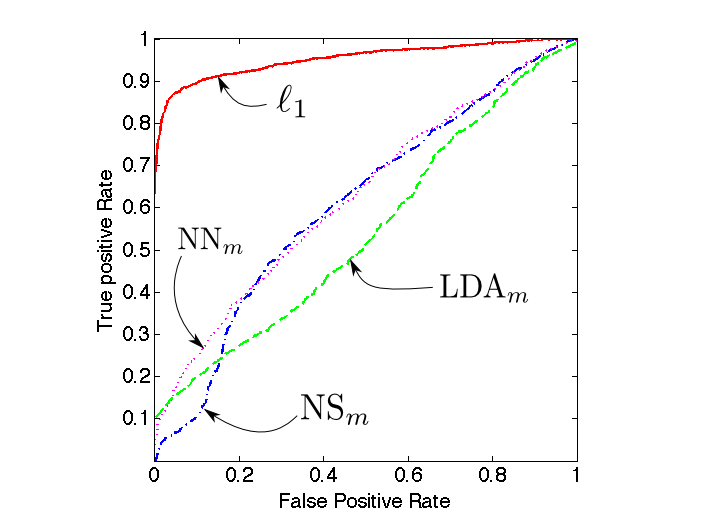
\includegraphics[width=5in]{figures_cvpr/roc3.png} 
}
\caption{{\bf Large-scale experiments on Multi PIE.} {\bf Top:} Recognition rates; {\bf Bottom:} ROC curves for our algorithm (labeled as ``$\ell_1$''), compared with those for NN$_m$, NS$_m$, and LDA$_m$.} \label{tab:multipie}
\end{figure}

\paragraph{Cause of errors.} Our algorithm's errors are mostly caused by a few subjects who significantly change their appearances between sessions (such as hair, facial hair, and eyeglasses). Some representative examples are shown in Figure \ref{fig:failed-examples}. In fact, for those subjects, alignment and recognition fail on almost all test illuminations.\vspace{0mm} %This may be due the limited number of illuminations present in the training. \vspace{0mm}
\begin{figure}
\centering
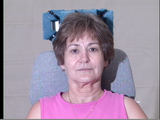
\includegraphics[scale=0.4,clip=true]{figures_cvpr/079_01_01_051_08.png} 
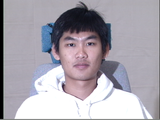
\includegraphics[scale=0.4,clip=true]{figures_cvpr/130_01_01_051_08.png} 
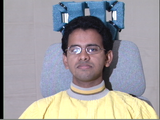
\includegraphics[scale=0.4,clip=true]{figures_cvpr/163_01_01_051_08.png} 
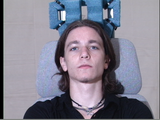
\includegraphics[scale=0.4,clip=true]{figures_cvpr/175_01_01_051_08.png} 
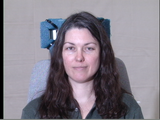
\includegraphics[scale=0.4,clip=true]{figures_cvpr/118_01_01_051_08.png} 
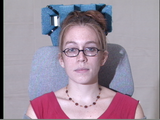
\includegraphics[scale=0.4,clip=true]{figures_cvpr/223_01_01_051_08.png} \\
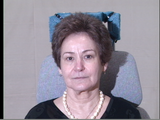
\includegraphics[scale=0.4,clip=true]{figures_cvpr/079_02_01_051_08.png} 
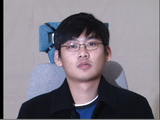
\includegraphics[scale=0.4,clip=true]{figures_cvpr/130_02_01_051_08.png} 
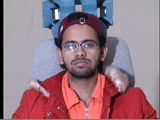
\includegraphics[scale=0.4,clip=true]{figures_cvpr/163_02_01_051_08.png} 
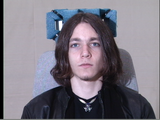
\includegraphics[scale=0.4,clip=true]{figures_cvpr/175_02_01_051_08.png} 
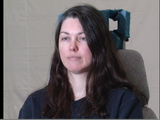
\includegraphics[scale=0.4,clip=true]{figures_cvpr/118_02_01_140_08.png} 
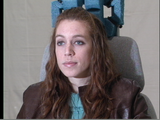
\includegraphics[scale=0.4,clip=true]{figures_cvpr/223_02_01_140_08.png} 
\caption{{\bf Representative examples of failed Multi-PIE subjects}. {\bf Top:} training from Session 1; {\bf Bottom:} test images from Session 2 -- first four are frontal and the last two with $15^\circ$ pose. Notice the change of hair style and facial hair, which makes alignment fail on those subjects, actually regardless of test image illuminations.\vspace{0mm}}\label{fig:failed-examples}
\end{figure}

\paragraph{Pose and expression.} We also run limited tests of our algorithm on images with pose and expression in Multi-PIE.  Using the same training as above, we test our algorithm on images in Session 2 with $15^\circ$ pose, for all 20 illuminations. The recognition rate is 77.5\%. We also test our algorithm on images in Session 3 with smile. For illumination 0 (ambient), the rate is 58.5\%, for illumination 10, the rate is 68.6\%.\vspace{0mm}


\subsection{Tests on our own datasets}\label{sec:own-data}\vspace{0mm}
Using the training acquisition system that we have described in the previous section, Figure \ref{fig:system}, we have collected the frontal view of 74 subjects {\em without eyeglasses} under 38 illuminations shown in Figure \ref{fig:illumination-patterns}. For testing our algorithm, we have also taken 593 images of these subjects with a different camera under a variety of practical conditions.\vspace{0mm}

\paragraph{Limitation of frontal illuminations.}
To see how training illuminations affect the performance of our algorithm in practice, we now compare how well a few frontal illuminations can interpolate: 1. other frontal illuminations taken under the same laboratory conditions, and 2. typical indoor and outdoor illuminations. To this end, we select 20 subjects from the face database acquired by our system and use 7 illuminations per subject as training. The illuminations are chosen to be similar to the 7 illuminations used in the previous experiment on Multi-PIE.\footnote{We use the illumination set $\{6, 9, 12, 13, 18, 21, 22\}$ shown in Figure \ref{fig:illumination-patterns}(b) to mimic the illumination set $\{0, 1, 6, 7, 13, 14, 18\}$ in Multi-PIE.} We then test our algorithm on the remaining $24 - 7 = 17$ frontal illuminations for all the 20 subjects. The recognition rate is $99.7\%$, nearly perfect. We also test our algorithm on $173$ frontal images of these subjects taken under a variety of indoor and outdoor conditions (in category 1 specified below), similar to the one shown in Figure \ref{fig:promo}, and the recognition drops down to $93.6\%$. One would expect the rate to drop even further when the number of subjects increases.\vspace{0mm}

\paragraph{Large-scale test with sufficient training illuminations.}
Now we use all 74 subjects and 38 illuminations in the training and test on 593 images taken under a variety of conditions. Based on the main variability in the test images, we have partitioned them into five main categories:%\vspace{0mm}
\begin{small}
\begin{description}
\item[C1:] 242 images of 47 subjects without eyeglasses, generally frontal view, under a variety of practical illuminations (indoor and outdoor) (Fig. 10, row 1). %\vspace{0mm}
\item[C2:] 109 images of 23 subjects with eyeglasses (Fig. 10, row 2).%\vspace{0mm}
\item[C3:] 19 images of 14 subjects with sunglasses (Fig. 10, row 3).%\vspace{0mm}
\item[C4:] 100 images of 40 subjects with noticeable expressions, poses, mild blur, and sometimes occlusion (Fig. 11, both rows).%\vspace{0mm}
\item[C5:] 123 images of 17 subjects with little control (out of focus, motion blur, significant pose, large occlusion, funny faces, extreme expressions) (Fig. 12, both rows).%\vspace{0mm}
\end{description}
\end{small}
We apply Viola and Jones' face detector on these images and directly use the detected faces as the input to our algorithm. The table below reports the performance of our algorithm on each category. The errors include failures of the face detector on some of the more challenging images.\vspace{0mm}
\begin{table}[h]	
\centering
\begin{tabular}{|l|c|c|c|c|c| }
\hline
Test Categories & C1 & C2 & C3 & C4 & C5  \\
\hline
\hline
Rec. Rates (\%) &  95.9 & 91.5 & 63.2 & 73.7 & 53.5 \\
\hline
\end{tabular} \vspace{0mm}
\end{table}

\begin{figure}
\centering
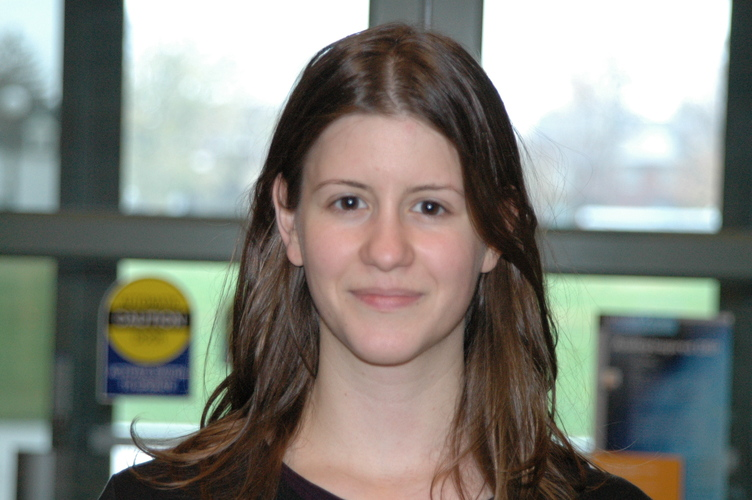
\includegraphics[scale=0.35,clip=true]{figures_cvpr/examples/1/DSC_1319.JPG} 
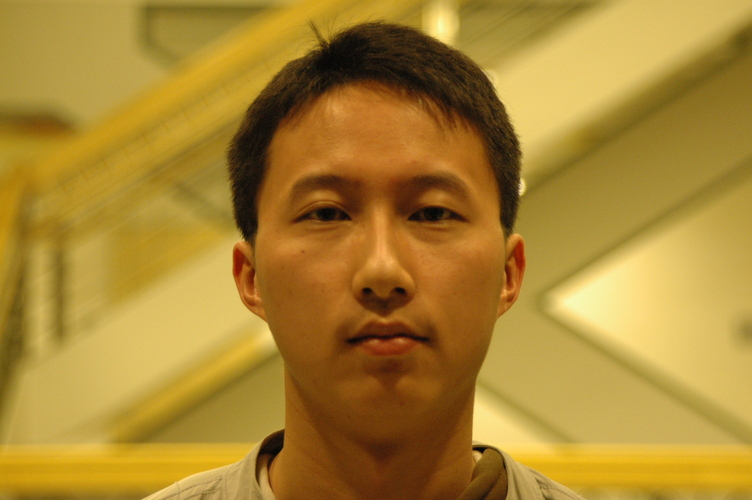
\includegraphics[scale=0.35,clip=true]{figures_cvpr/examples/1/DSC_1531.JPG} 
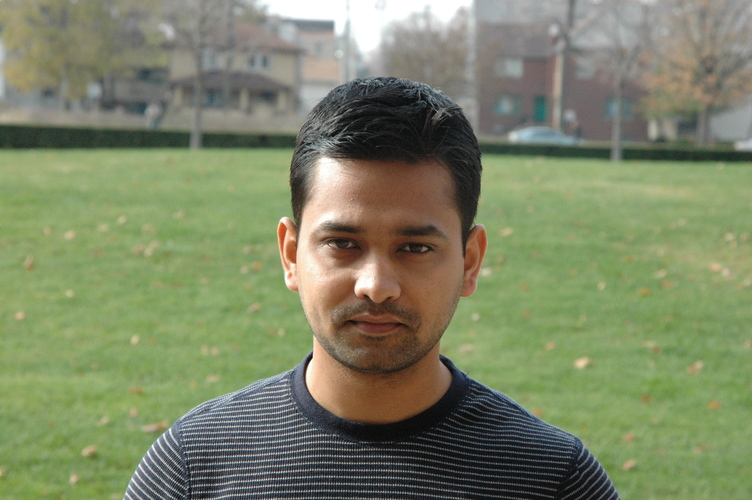
\includegraphics[scale=0.35,clip=true]{figures_cvpr/examples/1/DSC_1574.JPG} 
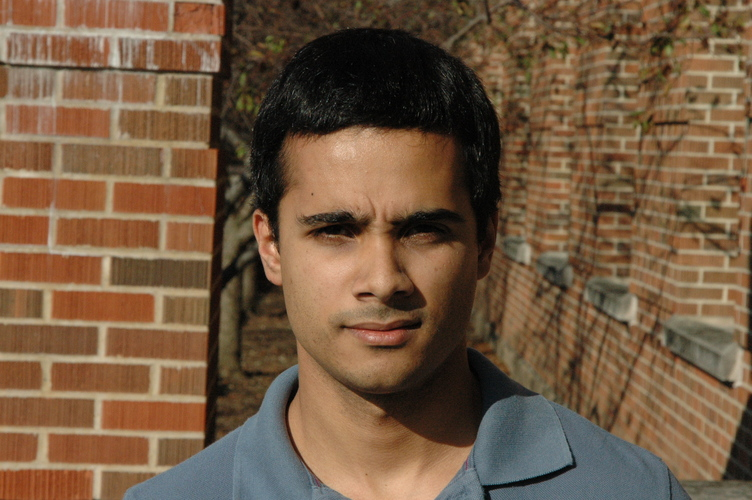
\includegraphics[scale=0.35,clip=true]{figures_cvpr/examples/1/DSC_1622.JPG} 
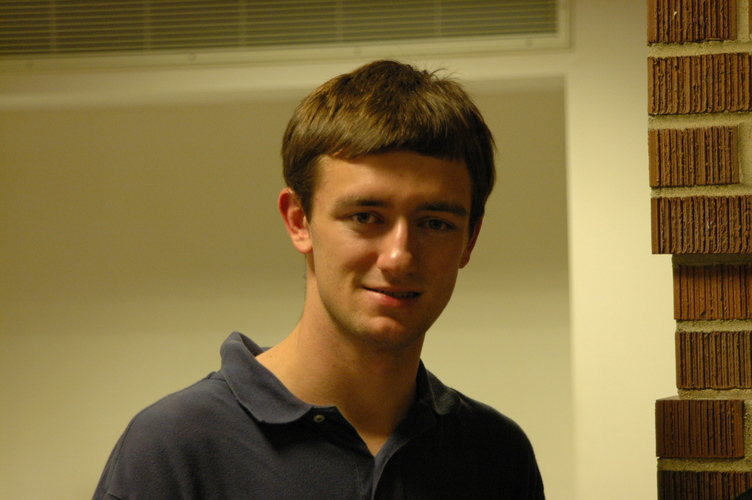
\includegraphics[scale=0.35,clip=true]{figures_cvpr/examples/1/DSC_1786.JPG} \\
\includegraphics[scale=0.35,clip=true]{figures_cvpr/examples/2/DSC_1448.JPG} 
\includegraphics[scale=0.35,clip=true]{figures_cvpr/examples/2/DSC_1585.JPG} 
\includegraphics[scale=0.35,clip=true]{figures_cvpr/examples/2/DSC_1588.JPG} 
\includegraphics[scale=0.35,clip=true]{figures_cvpr/examples/2/DSC_1666.JPG} 
\includegraphics[scale=0.35,clip=true]{figures_cvpr/examples/2/DSC_1874.JPG} \\
\includegraphics[scale=0.35,clip=true]{figures_cvpr/examples/3/DSC_1572.JPG} 
\includegraphics[scale=0.35,clip=true]{figures_cvpr/examples/3/DSC_1587.JPG} 
\includegraphics[scale=0.35,clip=true]{figures_cvpr/examples/3/DSC_1623.JPG} 
\includegraphics[scale=0.35,clip=true]{figures_cvpr/examples/3/DSC_1652.JPG} 
\includegraphics[scale=0.35,clip=true]{figures_cvpr/examples/3/DSC_1675.JPG} 
 \caption{{\bf Representative examples of categories 1-3}. One row for each category.\vspace{0mm}}\label{fig:examples1-3}
%\end{figure}
%\begin{figure}
\centering
\includegraphics[scale=0.35,clip=true]{figures_cvpr/examples/4/success/DSC_1579.JPG} 
\includegraphics[scale=0.35,clip=true]{figures_cvpr/examples/4/success/DSC_1839.JPG} 
\includegraphics[scale=0.35,clip=true]{figures_cvpr/examples/4/success/DSC_1883.JPG} 
\includegraphics[scale=0.35,clip=true]{figures_cvpr/examples/4/success/DSC_1922.JPG} 
\includegraphics[scale=0.35,clip=true]{figures_cvpr/examples/4/success/DSC_2000.JPG} \\
\includegraphics[scale=0.35,clip=true]{figures_cvpr/examples/4/failure/DSC_1568.JPG} 
\includegraphics[scale=0.35,clip=true]{figures_cvpr/examples/4/failure/DSC_1578.JPG} 
\includegraphics[scale=0.35,clip=true]{figures_cvpr/examples/4/failure/DSC_1500.JPG} 
\includegraphics[scale=0.35,clip=true]{figures_cvpr/examples/4/failure/DSC_1930.JPG} 
\includegraphics[scale=0.35,clip=true]{figures_cvpr/examples/4/failure/DSC_1985.JPG} 
 \caption{{\bf Representative examples of category 4}. Top row: successful examples. Bottom row: failures.}\label{fig:examples4}
\vspace{0mm}
\centering
\includegraphics[scale=0.35,clip=true]{figures_cvpr/examples/5/success/DSC_1664.JPG} 
\includegraphics[scale=0.35,clip=true]{figures_cvpr/examples/5/success/DSC_1777.JPG} 
\includegraphics[scale=0.35,clip=true]{figures_cvpr/examples/5/success/DSC_1871.JPG} 
\includegraphics[scale=0.35,clip=true]{figures_cvpr/examples/5/success/DSC_1913.JPG} 
\includegraphics[scale=0.35,clip=true]{figures_cvpr/examples/5/success/DSC_2005.JPG} \\
\includegraphics[scale=0.35,clip=true]{figures_cvpr/examples/5/failure/DSC_1669.JPG} 
\includegraphics[scale=0.35,clip=true]{figures_cvpr/examples/5/failure/DSC_1800.JPG} 
\includegraphics[scale=0.35,clip=true]{figures_cvpr/examples/5/failure/DSC_1870.JPG} 
\includegraphics[scale=0.35,clip=true]{figures_cvpr/examples/5/failure/DSC_1917.JPG} 
\includegraphics[scale=0.35,clip=true]{figures_cvpr/examples/5/failure/DSC_2008.JPG} 
 \caption{{\bf Representative examples of category 5}. Top row: successful examples. Bottom row: failures.\vspace{0mm}}\label{fig:examples5}
\end{figure}

\vspace{0mm}
\section{Conclusion}\vspace{0mm}
We have proposed a new algorithm and system for recognizing human faces from images taken under practical conditions. The proposed system is very {\em simple} and hence the results are easy to reproduce. The proposed algorithm is {\em scalable} both in terms of computational complexity and recognition performance. The system is directly compatible with off-the-shelf face detectors and achieves extremely {\em stable} performance under a wide range of variations in illumination, misalignment, pose, and occlusion. We achieve very good recognition performance on large-scale tests with public datasets and our practical face images, using only frontal 2D images in the training without any explicit 3D face model. 
%Our implementation still has plenty of room for further engineering improvements.\vspace{0mm}

%
%{\small
%\bibliographystyle{ieee}
%\bibliography{cvpr09_faces}
%}

%\end{document}


%!TEX root = thesis.tex

\chapter{IMPROVING ROBUSTNESS TO CONTINUOUS OCCLUSIONS}
\label{chap:iccv}

%\documentclass[10pt,twocolumn,letterpaper]{article}

%\usepackage{iccv}
%\usepackage{times}
%\usepackage{epsfig}
%\usepackage{graphicx}
%\usepackage{amsmath}
%\usepackage{amssymb}

%% Include other packages here, before hyperref.
%\usepackage{algorithm}
%\usepackage{algorithmic}

%% If you comment hyperref and then uncomment it, you should delete
%% egpaper.aux before re-running latex.  (Or just hit 'q' on the first latex
%% run, let it finish, and you should be clear).
%\usepackage[pagebackref=true,breaklinks=true,letterpaper=true,colorlinks,bookmarks=false]{hyperref}

%\renewcommand{\mathbf}{\boldsymbol}
%\renewcommand{\Re}{\mathbb{R}}
%\newcommand{\R}{\mathbb{R}}
%\newcommand{\E}{\mathbf{E}}
%\newcommand{\x}{\mathbf x}
%\newcommand{\y}{\mathbf y}
%\newcommand{\z}{\mathbf z}
%\renewcommand{\r}{\mathbf r}
%\newcommand{\e}{\mathbf e}
%\newcommand{\n}{\mathbf n}
%\newcommand{\G}{\mathbf G}
%\newcommand{\I}{\mathbf I}
%\renewcommand{\u}{\mathbf u}
%\newcommand{\s}{\mathbf s}

%\newtheorem{lemma}{Lemma}

%\newcommand{\jw}[1]{{\color{red} \bf John: #1}}

%\setlength\fboxsep{0pt}
%\setlength\fboxrule{0.5pt}

%
%% \iccvfinalcopy % *** Uncomment this line for the final submission

%\def\iccvPaperID{1145} % *** Enter the ICCV Paper ID here
%\def\httilde{\mbox{\tt\raisebox{-.5ex}{\symbol{126}}}}

%% Pages are numbered in submission mode, and unnumbered in camera-ready
%\ificcvfinal\pagestyle{empty}\fi
%\begin{document}

%%%%%%%%%% TITLE
%\title{Face Recognition With Contiguous Occlusion Using Markov Random Fields}

%\author{First Author\\
%Institution1\\
%Institution1 address\\
%{\tt\small firstauthor@i1.org}
%% For a paper whose authors are all at the same institution,
%% omit the following lines up until the closing ``}''.
%% Additional authors and addresses can be added with ``\and'',
%% just like the second author.
%% To save space, use either the email address or home page, not both
%\and
%Second Author\\
%Institution2\\
%First line of institution2 address\\
%{\small\url{http://www.author.org/~second}} }

%\maketitle
%% \thispagestyle{empty} % *** Uncomment this line for the final submission

%%%%%%%%% ABSTRACT
%\begin{abstract}
%Partially occluded faces are common in many applications of face
%recognition. While algorithms based on sparse
%representation have demonstrated promising results, they achieve their best performance on occlusions
%that are not spatially correlated (i.e.\ random pixel corruption). We show that such sparsity-based algorithms can be significantly improved by harnessing prior knowledge about the pixel error distribution. We
%show how a Markov Random Field model for spatial continuity of the occlusion can be integrated into the computation of a
%sparse representation of the test image with respect to the training images.
%Our algorithm efficiently and reliably identifies the
%corrupted regions and excludes them from the sparse representation.
%Extensive experiments on both laboratory and real-world datasets show that our algorithm tolerates much
%larger fractions and varieties of occlusion than current state-of-the-art algorithms. \vspace{0mm}
%\end{abstract}

\section{Introduction}
This chapter represents work that I performed in collaboration with Zihan Zhou, John Wright, Hossein Mobahi, and Yi Ma.  It is an extended version of a conference paper that has been submitted for review for the 2009 IEEE Conference on Computer Vision.  While the previous chapter provided the overall design for a complete face recognition system, the work described in this chapter focuses on improving the robustness of the face recognition algorithm to occlusion.

Occlusion is a common difficulty encountered in applications of automatic face recognition. Sources of occlusion include apparel such as  eyeglasses, sunglasses, hats, or scarves, as well as objects such as cell phones placed in front of the face. Moreover, even in the absence of an occluding object, violations of an assumed model for face appearance may act like occlusions: e.g., shadows due to extreme illumination violate the assumption of a low-dimensional linear illumination model \cite{Basri2003-PAMI}. Robustness to occlusion is therefore essential to practical face recognition.

If the face image is partially occluded, popular recognition algorithms based on holistic features such as Eigenfaces and Fisherfaces \cite{Turk1991-CVPR,Belhumeur1997-PAMI} are no longer applicable, since all of the extracted features will be corrupted. If the spatial support of the occlusion can be reliably determined (e.g., using features such as color \cite{Jia2008-FGR,Jia2009-CVPR}), the occluded region can be discarded and recognition can proceed on the remaining part of the image. However, if the spatial support of the occlusion is initially unknown, one traditional approach is to rely on spatially localized features such as local image patches \cite{Martinez-02,Pentland1994-CVPR,Ahonen2006-PAMI}, or randomly sampled pixels \cite{Leonardis2000-CVIU,Fidler2006-PAMI}. Data-dependent spatially localized bases can also be computed using techniques such as independent component analysis (ICA) or localized nonnegative matrix factorization (LNMF) \cite{KimJ2005-PAMI,LiS2001-CVPR}. Clearly, such local features are less likely to be corrupted by partial occlusion than holistic features. However, as observed in \cite{Wright2009-PAMI}, operating on a small set of local features could discard useful redundant information in the test image, which is essential for detecting and correcting gross errors.

To avoid losing useful information with local feature extraction, \cite{Wright2009-PAMI} casts face recognition as the problem of finding a sparse representation of the entire test image in terms of the training images, except for a sparse portion of the image that might be corrupted due to occlusion.
The $n_i$ frontal\footnote{In \cite{Wright2009-PAMI}, both the training and test data are assumed to be well-registered frontal images. We also make this assumption, in order to isolate the effect of occlusion.} training images of each subject $i$ under
varying illuminations are stacked as columns of a matrix $A_i \in \R^{m\times n_i}$. Concatenating the training images of all $K$ subjects gives a large matrix $A = [A_1,A_2,\ldots,A_K] \in \R^{m\times n}$, ($n = \sum_i n_i$).
\cite{Wright2009-PAMI} then represents the given test image $\y \in \Re^m$ as a sparse linear
combination $A \x$ of all images in the data set, plus a sparse error
$\e$ due to occlusion: $\y = A \x + \e$. The sparse coefficients $\x$ and sparse error $\e$ are recovered by solving the $\ell^1$-norm minimization problem
\begin{equation}
\min \|\x\|_1 + \|\e\|_1\quad \textup{s.t.} \quad \y = A \x + \e.
\end{equation}
This approach has demonstrated good potential in handling occlusion, especially when the dimension of the image signal is high \cite{Wright2008-IT}. Experiments in \cite{Wright2009-PAMI} showed that the algorithm can tolerate up to 70\% random pixel corruption or 40\% random block occlusion while still maintaining recognition rates higher than $90\%$ on the Yale B database.

However, in experiments on face images the $\ell^1$-minimization algorithm is not nearly as robust to contiguous occlusion as it is to random pixel corruption.  On the AR database sunglasses and scarf occlusions it achieves only 87\% and 59.5\% respectively.  This algorithm does not exploit any prior information about the corruption or occlusion (it is invariant to pixel ordering).  To try to improve performance for these cases, \cite{Wright2009-PAMI} proposed to partition the image into blocks and compute an independent sparse representation for each block. This significantly improves the recognition rates (up to 97.5\% and 93.5\% respectively). However, such fixed partition schemes only work for limited types of occlusion, and are less likely to scale well to large databases, since they essentially treat small image blocks independently.

In this chapter, we propose a more principled and general method for face recognition with {\em contiguous} occlusion. We do not assume any explicit prior knowledge about the location, size, shape, color, or number of the occluded regions; the only prior information we have about the occlusion is that the corrupted pixels are likely to be adjacent to each other in the image plane. The goal of this chapter is to show how to effectively incorporate this prior information into the sparse representation framework, significantly improving its robustness to all types of realistic occlusions.

\section{Motivation for imposing local spatial continuity for sparse error correction}
Before introducing a model for the contiguous occlusion and incorporating it into a solution for face recognition, let us first justify why imposing spatial continuity could potentially help with finding the sparse errors (in our case, the occluded pixels). As discussed above, face recogntion can be cast as a problem of recovering an input signal $\x\in \R^n$ from corrupted measurements $\y = A\x+\e$, where $A\in
\Re^{m\times n}$ with $m>n$. Let $F$ be a matrix whoose rows span the left nullspace of
$A$\footnote{$\mathrm{rank}(F) = m - \mathrm{rank}(A)$ and $FA=0$}. Applying $F$ to both sides of the measurement equation gives \vspace{0mm}
\begin{displaymath}
\tilde{\y} \doteq F \y = F(A \x+ \e) = F\e. \vspace{0mm}
\end{displaymath}
So the recovery problem is reduced to the problem of reconstructing
a sparse error vector $\e$ from the observation $F \e$. While this problem is very hard in general, in many situations solving the convex relaxation \vspace{0mm}
\begin{equation*}
\min \| \mathbf{v} \|_1 \quad \textup{s.t.} \quad F \mathbf{v} = \tilde{\y} = F \e \vspace{0mm}
\end{equation*}
exactly recovers $\e$.

Candes et.\ al.\ \cite{CandesE2005-IT} have characterized the recoverability of the sparse solution to the above problem in terms of the {\em restricted isometry property} (RIP) of the matrix $F$.
The $k$-restricted isometry constant $\delta_k \in \Re$ is defined as the smallest
quantity such that for any $k$-sparse $\x$,
\begin{equation}
(1-\delta_k)\|\x\|_2 \leq \|F\x\|_2 \leq (1+\delta_k)\|\x\|_2.
\label{eq-rip}
\end{equation}
A typical result states $\ell^1$-minimization is guaranteed to recover any $k$-sparse $\x$ whenever the matrix
$F$ satisfies $\delta_{2k}<1$. Notice that this argument treats every
possible $k$-sparse supports equally. However, in many
applications, we have prior information about the
distribution of the supports. To extend the theory to such
structured sparsity, \cite{Cevher2008-NIPS} introduced the
$(k,\epsilon)$-probabilistic RIP (PRIP). A matrix $F$ is said to
satisfy the PRIP if there exists a constant $\delta_k>0$ such that
for a $k$-sparse signal $\x$ whose support is a considered as a random variable, \eqref{eq-rip} holds with probability $\ge 1-\epsilon$.

Based on results from Compressed Sensing theory, for a randomly chosen matrix to have RIP of order $k$ requires at least $m =\mathcal{O}(k\log(n/k))$ measurements \cite{CandesE2005-IT}. However, it has been shown that a matrix can have PRIP of order $k$ with only $m =\mathcal {O}(k + \log(D))$ measurements, where $D$ is the cardinality of the smallest set of supports of size $k$ for which the probability that the support of a $k$-sparse signal $\x$ does not belong to the set is less than $\epsilon$ \cite{Cevher2008-NIPS}. Then for distributions that allow a small $D$, the required number of measurements essentially grows linearly in $k$, much less than the general case. The distribution of contiguous supports precisely falls into this category\footnote{Simple counting arguments similar to that in \cite{Cevher2008-NIPS} indicate that $D$ can be upper-bounded by a polynomial of the dimension $m$.}. Thus, we should expect to recover sparse errors with such supports from much fewer measurements. Or equivalently, from a fixed number measurements, we should expect to correct a larger fraction of errors from $\ell^1$-minimization {\em if} we know how to properly harness information about the distribution.

\section{Using a Markov random field assumption to impose local spatial continuity of the error support}
Consider the error vector $\e\in \R^m$ incurred by some contiguous occlusion. Its nonzero entries should be both sparse and spatially continuous. Given an error vector $\e\in \R^m$, we let $\s\in \{-1,1\}^m$ denote its
support vector. That is, $\s[i] = -1$ when $\e[i] = 0$ and $\s[i] = 1$
when $\e[i] \neq 0$. The image domain can be considered as a graph
$G=(V,E)$, where $V = \{1,\dots,m\}$ denotes the set of $m$
pixels and $E$ denotes the edges connecting neighboring pixels.

The spatial continuity among the corrupted pixels (and also the uncorrupted pixels as well) can then be modeled by a Markov random field (MRF). We adopt the classical {\em Ising model} for the probability mass function of error supports $\s$:
\begin{equation}
p(\s) \propto \exp\Bigl\{\sum_{(i,j)\in
E}\lambda_{ij}\s[i]\s[j] + \sum_{i\in V}\lambda_i \s[i]\Bigr\}.
\label{eqn:ising}
\end{equation}
Here, $\lambda_{ij}$ controls the interaction between support values $\s[i]$ and $\s[j]$ on neighboring pixels and $\lambda_i$ indicates any prior information about the supports. In this implementation, we fix $\lambda \ge 0$ and let \vspace{0mm}
\begin{displaymath}
{\lambda}_{ij} = \lambda \;\forall\,(i,j) \in E, \quad \mbox{and} \quad \lambda_i = 0 \;\,\forall\;i. \vspace{0mm}
\end{displaymath}
The first condition means that each pair of neighboring pixels exert the same influence on each other, while the second condition indicates that we do not make any additional prior assumptions about the locations of the erroneous pixels.

\begin{figure} 
\centerline{\includegraphics[width=4.0in]{figures_iccv/function.pdf}}
\caption{Approximation to the likelihood of $\e$ given the error support. Left: $p(\e|\s = -1)$ (unoccluded pixels). Right: $p(\e|\s = 1)$ (occluded pixels).} \label{fig:likelihood} \vspace{0mm}
\end{figure}

The Ising model makes the fundamental assumption that the pixel values are independent of each other given the support. Hence we can write down the joint probability density function of the error vector $\e$ in exponential form as:
\begin{eqnarray*}
p(\e,\s) &=& p(\s) p(\e|\s) \,=\, p(\s) \prod_i p(\e[i]|\s[i]) \\
&\propto&  \exp\Big\{\hspace{-2mm}\sum_{(i,j)\in E} \hspace{-2mm}\lambda\s[i]\s[j] +
\sum_{i\in V} \log p(\e[i] \mid \s[i]) \Big\}.
\end{eqnarray*}
We normalize the range of error values to $[0,1]$, and approximate the log-likelihood function $\log p(\e[i]\mid\s[i])$ as follows:
\begin{eqnarray*}
\log p(\e[i] \mid \s[i]=-1) &=& \left\{ \begin{array}{ll}
-\log \tau & \textrm{if $|\e[i]| \le \tau$},\\
\log \tau & \textrm{if $|\e[i]| >\tau$},
\end{array} \right. \\
\log p(\e[i] \mid \s[i]=1) &=& \left\{ \begin{array}{ll}
0 & \textrm{if $|\e[i]| > \tau$},\\
\log \tau & \textrm{if $|\e[i]| \le \tau$}.
\end{array} \right.
\end{eqnarray*}
This corresponds to the piecewise-constant likelihood function $p(\e\mid \s)$ pictured in Figure \ref{fig:likelihood}. While the precise form of the approximation is not essential to the success of the method, in this model $\tau$ effectively acts as a threshold for considering pixels as errors, subject to the spatial continuity prior. The constant $\tau$ should be set so that it is larger than the noise level and within-class variability of the non-occluded pixels, but smaller than the magnitude of the errors due to occlusion.  In Section \ref{sec:tau} we will see how this threshold can be chosen adaptively without prior knowledge of the statistics of the training and test images.

\subsection{Error correction with both MRF and sparsity}
Now consider an image $\y$ of subject $k$. Without occlusion, it can be well-approximated as a linear combination of training images of the same subject: $\y = A_k \x_k$. If, however, a portion of the image is occluded, we need to discard that portion in order for the same linear equation to hold. Thus, a natural goal is to identify the most likely portion  on which $\y = A_k \x_k$ holds for some $\x_k$. In terms of the error model introduced above, we want to solve the following optimization problem:
\begin{equation}
\hat \s = \mbox{arg}\max_{\x_k,\e,\s} p(\s, \e) \quad \mbox{s.t.} \quad \y = A_k \x_k + \e.
\end{equation}
This is a difficult nonconvex optimization problem in many variables $\s, \e, \x_k$. We will locally optimize this objective function by iterating between estimating the support $\s$ and estimating the regressor $\x_k$, with the other fixed.

\paragraph{1. Estimating Linear Regressor $\x_k$ with Sparsity.}
Given an initial estimate of the error support $\s$,\footnote{We initialize the algorithm with empty error support ($\s = -1$).} we simply exclude that part, and use the rest of the image to estimate the linear regressor $\x_k$. Let $A_k^*$ and $\y^*$ denote $A_k$ and $y_k$ with the rows marked as occlusion ($\s = -1$) removed.
If estimate of $\s$ was exactly correct, then we would have $\y^* = A_k^* \x_k$ for some $\x_k$, and could simply estimate $\x_k$ by linear regression. However, it is more reasonable to assume that the intermediate estimate of the support $\s$ could be wrong in a subset of its entries, and some pixels in $\y^*$ might be still corrupted. If $\s$ is a reasonable guess, however, these violations will be relatively few and we can estimate $\x_k$ via the following convex program:
\begin{equation}
(\hat{\x}_k,\hat{\e}^*) = \arg\min \|\e^*\|_1  \; \textup{ s.t. } \; \y^* = A_k^*\x+\e^*, \x\geq
0.
\end{equation}
That is, we look for a regressor $\x_k$ such that the $\ell^1$-norm of the error $\e^*$ is minimized. The complete error vector $\e \in \Re^m$ can then be estimated as $\hat \e = \y - A \hat{\x}_k$.

\paragraph{2. Estimating Error Support $\s$ with MRF.} 
Given an initial estimate of the regressor $\x_k$ and corresponding estimate of the error vector $\e = \y - A \x_k$, we may re-estimate the support vector $\s$ as the one that maximizes the log likelihood $\log p(\e,\s)$:\vspace{0mm}
\begin{equation}
\hat{\s} = \arg\hspace{-2mm}\max_{\s \in \{-1,1\}^m}\hspace{-2mm} \sum_{(i,j)\in E} \hspace{-2mm} \lambda \s[i]\s[j] +
\sum_{i\in V} \log p(\e[i] | \s[i]). \vspace{0mm}
\end{equation}
This is an integer programming problem, but due to the special structure of the Ising model, it can be solved exactly in linear time, using graph cuts \cite{Kolmogorov2004-PAMI}.

\vspace{1 em}
Empirically, we observe that the above iteration between steps {\bf1.} and {\bf2.} converges in about five or six iterations. Once we have obtained final estimates of the error support $\s$, error values $\e$, and regressors $\x$, we still need to identify the subject based on some measure of goodness-of-fit within the unoccluded region. Here, we choose to assign the test image to the class that minimizes the $\ell^1$-error in that region, divided by the square of the number of unoccluded pixels:\vspace{0mm}
$$\text{identity}(\y) = \arg \min_k \; \frac{\| \y^* - A_k^* \x_k \|_1}{|\{ i \mid \s_k[i] = -1 \}|^2}. \vspace{0mm}$$
Here, squaring encourages the algorithm to choose solutions with as few occluded pixels as possible.
%While the precise form of the classification heuristic is less important than the correct estimation of the occlusion, we note in passing that the scaling is correct: both the numerator and denominator are linear in the number of image pixels.

We summarize the overall procedure as Algorithm 1 below. Since this algorithm operates on each subject's images individually, the overall complexity is linear in the number of subjects. Moreover, with fast implementations of both $\ell^1$-minimization and graph cuts,\footnote{Our implementation of $\ell^1$-minimization is a custom interior point method, while the graph cuts are computed with package of \cite{Boykov2001-PAMI,Kolmogorov2004-PAMI,Boykov2004-PAMI}, downloaded from \url{http://www.csd.uwo.ca/~olga/code.html}.} the computation time per subject is fairly small. On a Dual-Core Intel Xeon 2.66GHz computer, with 19 training images of resolution $96 \times 84$ per subject, our C++ implementation requires approximately 0.3 seconds per subject.

\begin{algorithm}[h]
\caption{{\bf (Sparse Error Correction with MRF)}} \label{alg:p-mrf}
\begin{algorithmic}[1]
\STATE {\bf Input:} A matrix of normalized training samples $A =
[A_1,A_2,\ldots,A_K] \in \Re^{m\times n}$ for $K$ classes, a test
sample $\y \in \Re^{m}$.

\FOR{each subject $k$}

\STATE Initialize the error support $\s^{(0)}_k = \mathbf{-1}_m$.

\STATE {\bf repeat}

\STATE \hspace{3mm}$A_k^* = A_k[\s^{(t-1)}_k=-1,\, :\, ]$, $\y^* =
\y[s^{(t-1)}_k=-1]$;

\STATE \hspace{3mm}Solve the convex program\\
\hspace{5mm} $(\hat{\x}_k,\hat{\e}^*) \;=\; \arg\min \|\e^*\|_1 $\\
\hspace{24mm} $\mathrm{ s.t. } \quad \y^* = A_k^*\x+\e^*, \, \x\geq 0;$

\STATE \hspace{3mm}$\hat{\e}_k\leftarrow \y-A_k\hat{\x}_k$;

\STATE \hspace{3mm}Update error support via graph cuts:\vspace{0mm}
$$\s^{(t)}_k = \arg\hspace{-4mm}\max_{\s\in\{-1,1\}^m}\hspace{-2mm}\sum_{i,j\in
E}\hspace{-2mm}{\lambda} \s[i]\s[j]+\sum_{i\in
V}\log\big(p(\hat{\e}_k[i]|\s[i])\big);$$\vspace{0mm}
\STATE {\bf until} maximum iterations or convergence.

\STATE Compute the normalized error $$\mathbf{r}_k(\y) =
\frac{\|\y^*-A_k^*\hat{\x}_k\|_1}{|\{ i \mid \s_k[i] = -1 \}|^2}. \vspace{0mm}$$
\ENDFOR

\STATE {\bf Output:} identity$(\y) = \arg\min_k \r_k(\y)$.
\end{algorithmic}
\end{algorithm}

\begin{figure*}[t]
\centering
{\small
\begin{tabular}{cccccccc}
\fbox{\includegraphics[height=0.8in]{figures_iccv/test_epsilon.png}}&
\fbox{\includegraphics[height=0.8in]{figures_iccv/epsilon3/20.png}}&
\fbox{\includegraphics[height=0.8in]{figures_iccv/epsilon3/17.png}}&
\fbox{\includegraphics[height=0.8in]{figures_iccv/epsilon3/14.png}}&
\fbox{\includegraphics[height=0.8in]{figures_iccv/epsilon3/11.png}}&
\fbox{\includegraphics[height=0.8in]{figures_iccv/epsilon3/8.png}}&
\fbox{\includegraphics[height=0.8in]{figures_iccv/epsilon3/5.png}}&
\fbox{\includegraphics[height=0.8in]{figures_iccv/epsilon3/2.png}}\\
&
\fbox{\includegraphics[height=0.8in]{figures_iccv/epsilon1/20.png}}&
\fbox{\includegraphics[height=0.8in]{figures_iccv/epsilon1/17.png}}&
\fbox{\includegraphics[height=0.8in]{figures_iccv/epsilon1/14.png}}&
\fbox{\includegraphics[height=0.8in]{figures_iccv/epsilon1/11.png}}&
\fbox{\includegraphics[height=0.8in]{figures_iccv/epsilon1/8.png}}&
\fbox{\includegraphics[height=0.8in]{figures_iccv/epsilon1/5.png}}&
\fbox{\includegraphics[height=0.8in]{figures_iccv/epsilon1/2.png}}\\
& (a) & (b) & (c) & (d) & (e) & (f) & (g)
\end{tabular}
}
\caption{Effect of $\tau$. Left: test image from AR database, occluded by scarf.
Right: estimated error supports for varying $\tau$. First row: $\lambda = 3$. Second row:
$\lambda = 1$. (a) $\tau=0.2$, (b) $\tau=0.17$, (c)
$\tau=0.14$, (d) $\tau=0.11$, (e) $\tau=0.08$, (f)
$\tau=0.05$, (g) $\tau=0.02$.} \label{fig:epsilon} \vspace{0mm}
\end{figure*}

\vspace{0mm}
\subsection{Choosing $\tau$} \label{sec:tau}

The parameter $\tau$ in the Ising model indicates the level
of error we would accept before considering an entry of the image as occluded. We
normalize the error value to be in the range $[0,1]$, so $\tau$
should also be chosen in $[0,1]$. This is not an easy
task for at least three reasons. First, it is sensitive to the
choice of the other parameter of MRF, $\lambda$. Figure
\ref{fig:epsilon} shows the estimate of error supports for a face
image with scarf occlusion versus different values of $\tau$.
With $\lambda = 3$, we can set $\tau=0.05$ and obtain almost perfect
identification of occluded area, but this is not true if $\lambda =
1$; in this case we obtain many false positives. Second, the choice of
$\tau$ depends on the level of noise and within-class variation in the
training and testing data. Third, the initial solution to
the $\ell^1$-minimization problem may be somewhat unreliable in the
presence of large amounts of occlusion.
In this case, starting with a small $\tau$ will result in many pixels being
falsely labelled as occluded early in the iteration.

We therefore choose $\tau$ adptively, starting with a
relatively large value, reducing it by a constant step size
at each iteration. We base our stopping criterion on the observation that for many test images, there is a
range of $\tau$ over which the estimate of $\s$ is stable.
For example, in Figure \ref{fig:epsilon}, any $\tau$ between 0.2 and 0.05 is good; in
the second row of Figure \ref{fig:epsilon}, any $\tau$ between
0.17 and 0.11 is good. As shown in Figure \ref{fig:epsilon}(g) and
Figure \ref{fig:n_goodentry}, this stable range is followed by a sudden drop in the
number of pixels considered unoccluded when $\tau$ falls below a certain critical value.
For our algorithm, we start with $\tau_1 = 0.17$. At the $i$th
iteration, we set $\tau_i = \tau_{i-1}-0.03$. Let $N_i$
denote the number of good entries at $i$th iteration. We stop
decreasing $\tau$ when $N_i < k \times N_{i-1}$, i.e. when there is a sudden increase in occluded pixels.  $k$ is an
empirically chosen constant, which we set to $0.4$ in our experiments.
After fixing $\tau$, we allow the algorithm to continue iterating
between estimating $\x$ and estimating $\s$ until convergence.

\begin{figure}
\centering
\includegraphics[scale=0.6,clip=true]{figures_iccv/n_of_goodentry.pdf}\vspace{2mm}
\caption{Number of entries estimated as unoccluded versus
$\tau$ for the sequence of images in the first row in figure \ref{fig:epsilon}. The {\bf \textcolor{red} o} indicates the
point at which the algorithm detects a sudden drop and stops
decreasing $\tau$.} \label{fig:n_goodentry} \vspace{0mm}
\end{figure}

\subsection{Effect of $\lambda$}

The parameter $\lambda$ in the Markov random field model controls
the strength of mutual interaction between adjacent pixels. Hence, it
should correspond to the smoothness level of error supports for
each individual test image. Note that for $\lambda=0$, maximizing
the probability of the Ising model reduces to simply thresholding
based on $\tau$, and our algorithm becomes similar in spirit to
reweighted $\ell^1$-minimization \cite{Candes2008-JFAA}, but
with a nonlinear reweighting step that more agressively discounts occluded pixels.

We will see that even simple thresholding works
quite well in cases where the occlusion the is uncorrelated with the face and
hence relatively easy to distinguish. This is especially true when the
image resolution (i.e., the number of measurements) is high.
With fewer measurements, however, enforcing prior
information about the spatial continuity of the error supports by
properly choosing $\lambda$ is essential.\vspace{0mm}


\section{Simulations and Experiments} \label{sec:experiments}

In this section, we conduct experiments using three publicly available databases. Using the Extended Yale B database \cite{Georghiades2001-PAMI,Lee2005-PAMI}, we will investigate the breakdown point of our algorithm under varying levels of (synthetic) contiguous occlusion. In this setting, the algorithm maintains high recognition rates up to 80\% occlusion. Then with AR Face database \cite{Martinez1998-report}, we will show that this good performance carries over to more realistic occlusions such as sunglasses and scarves, and furthermore, that by exploiting knowledge of the spatial distribution of the occlusion, one can recover an occluded face from far fewer measurements (i.e., lower resolution images). Finally, we test algorithm with a database obtained from the authors of  \cite{Wagner2009-CVPR}, which contains multiple categories of occluded test images taken under realistic illumination conditions. \vspace{-0mm}

\begin{figure}
\centering
{\small
\begin{tabular}{cccc}
\fbox{\includegraphics[height=0.8in]{figures_iccv/yale_exp/1/y.png}}&
\fbox{\includegraphics[height=0.8in]{figures_iccv/yale_exp/1/e.png}}&
\fbox{\includegraphics[height=0.8in]{figures_iccv/yale_exp/1/L.png}}&
\fbox{\includegraphics[height=0.8in]{figures_iccv/yale_exp/1/y_rec.png}}\\
&
\fbox{\includegraphics[height=0.8in]{figures_iccv/yale_exp/2/e.png}}&
\fbox{\includegraphics[height=0.8in]{figures_iccv/yale_exp/2/L.png}}&
\fbox{\includegraphics[height=0.8in]{figures_iccv/yale_exp/2/y_rec.png}}\\
&
\fbox{\includegraphics[height=0.8in]{figures_iccv/yale_exp/6/e.png}}&
\fbox{\includegraphics[height=0.8in]{figures_iccv/yale_exp/6/L.png}}&
\fbox{\includegraphics[height=0.8in]{figures_iccv/yale_exp/6/y_rec.png}}\\
(a) & (b) & (c) & (d)
\end{tabular}
}
\caption{Recovering a face image in Yale database from synthetic occlusion with $\lambda = 3$. Top: first iteration, Middle: second iteration, Bottom: final
result. (a) Test image
with 60\% occlusion. (b) Estimated error $\e$. (c) Error support estimated by
graph cuts. (d) Reconstruction
result.} \label{fig:yale_exp} \vspace{0mm}
\end{figure}


\paragraph{Recognition with synthetic occlusion.}

For this experiment, we use the Extend Yale B database to test the
robustness of our algorithm to synthetic occlusion. Among 1238
frontal face images of 38 subjects under varying laboratory lighting
conditions in Subset 1, 2 and 3 of Extended Yale B database, we
choose four illuminations from Subset 1 (mild illuminations), two
from Subset 2 (moderate illuminations) and two from Subset 3
(extreme illumiations) for testing and the rest for training. The
total numbers of images in training and testing sets are 935 and 303,
respectively. The images are cropped to $96 \times 84$ pixels.

To compare our method with the algorithm in \cite{Wright2009-PAMI}, we simulate various levels of contiguous occlusion from 10\% to 90\%
by replacing a random located block of a face image with the image of a baboon.
Figure \ref{fig:yale_exp}(a) shows an example of a 60\%
occluded face image. Figure \ref{fig:yale_exp}(c) illustrates the
iterative estimates of the error supports with $\lambda=3$.
For this test image, convergence occurs after six iterations.

We compare our result to the algorithm in \cite{Wright2009-PAMI} as
well as other baseline linear projection based algorithms, such as
Nearest Neighbor (NN), Nearest Subspace (NS) and Linear Discriminant
Analysis (LDA). Since these algorithms do not consider the special
structure of the error supports, they are not expected to work well
for high levels of occlusion. For this
experiment, we choose $\lambda=3$ for our algorithm. The results for
our algorithm are listed in Table \ref{tab:res-yale}. We compare the
results of all five algorithms in Figure \ref{fig:yale_result}(a).
Up to 70\% occlusion, our algorithm performs almost perfectly, while
the recognition rates for all the other algorithms fall below 50\%.
Even with 80\% occlusion, only 11.5\% of images are misclassified.
This is quite surprising because to the human eye, a face image
is barely recognizable if the block occlusion is more than 60\%.\vspace{0mm}
\begin{table*}[th]
{\centerline {\small
\begin{tabular}{|c|c|c|c|c|c|c|c|c|c|}
\hline
Percent occluded & 10\% & 20\% & 30\% & 40\% & 50\% & 60\% & 70\% & 80\% & 90\%\\
\hline
Recognition rate & 100\% & 100\% & 100\% & 100\% & 100\% & 100\% & 99.7\% & 88.5\% & 40.3\%\\
 \hline
\end{tabular}
}} \vspace{0mm} \caption{Recognition rates on the Extended Yale B dataset with varying level
of synthetic occlusion ($\lambda=3$).} \label{tab:res-yale} \vspace{0mm}
\end{table*}
\begin{figure}
\centering
\centerline{\small
\begin{tabular}{cc}
\includegraphics[height=2.2in]{figures_iccv/results/yale_cmp.pdf} & \hspace{-.35in}
\includegraphics[height=2.2in]{figures_iccv/results/yale_lambda.pdf}\\
(a) & (b)
\end{tabular}
}
\caption{Recognition with synthetic occlusion on the Yale dataset. (a) The recognition
rate for various algorithms with 10\% to 90\% occlusion. Our
algorithm remains perfect at 70\% occlusion while all the other
algorithms drop below 50\%. (b) Results of our algorithm with
different choices of $\lambda$. }\label{fig:yale_result} \vspace{0mm}
\end{figure}

In Figure \ref{fig:yale_result}(b) we show the results of our
algorithm for $\lambda = 0,1,2,3,5$. All the choices work
upto 80\% occlusion with above 80\% recognition rates.
However, compared to setting $\lambda=0$ and ignoring the spatial structure of the
error, enforcing continuity by setting $\lambda = 3$
results in an 8\% increase in recognition rate for the 80\% occlusion case.

Finally, instead of using a single block as occlusion, we test our
algorithm with occlusion by multiple small blocks. We consider three block sizes,
$8 \times 8$, $16\times 16$, and $32 \times 32$. For each fixed block
size, we add blocks to random selected locations of the
original face images until the total amount of coverage achieves a
desired occlusion level. Example test images for each block
size are shown in Figure \ref{fig:test_sample}. 
Table \ref{tab:res-block} reports the recognition rate as a function of 
block size and $\lambda$. Notice that $\lambda = 2$ provides uniformly 
good results ($> 92\%$ recognition for all cases). As expected, for small $\lambda$ the recognition 
performance decreases with increasing spatial continuity (block size), 
while for large $\lambda$ the recognition performance improves as the block size increases.\vspace{0mm}
\begin{figure}
\centering
{\small
\begin{tabular}{ccc}
\fbox{\includegraphics[height=1.0in]{figures_iccv/test_samples/32by32.png}}&
\fbox{\includegraphics[height=1.0in]{figures_iccv/test_samples/16by16.png}}&
\fbox{\includegraphics[height=1.0in]{figures_iccv/test_samples/8by8.png}}\\
(a) & (b) & (c)
\end{tabular}
}
\caption{Test images with multiple-block occlusion. (a) $32\times 32$ blocks.
(b) $16\times 16$ blocks. (c) $8 \times 8$ blocks. All images are 80\% occluded.}\label{fig:test_sample} \vspace{0mm}
\end{figure}
\begin{table}[ht]
{\centerline {\small
\begin{tabular}{|c|c|c|c|c|c|}
\hline
Block Size & $\lambda=0$ & $\lambda=1$ & $\lambda=2$ & $\lambda=3$ & $\lambda=5$\\
\hline
$32 \times 32$ & 89.4 & 88.8 & {\bf 92.7} & 86.5 & 68.6\\
 \hline
$16 \times 16$ & 92.1 & 93.7 & {\bf 93.7} & 85.8 & 68.65\\
 \hline
$8 \times 8$ & 90.4 &  94.4  &  {\bf 96.0}  &  85.2  &  29.7 \\
 \hline
\end{tabular}
}} \vspace{0mm} \caption{Recognition rates with 80\% occlusion by multiple blocks.} \label{tab:res-block} \vspace{0mm}
\end{table}

\paragraph{Recognition with disguises.}

We next test our algorithm on real disguises using a subset of the
AR Face Database. The training set consists 799 unoccluded face
images of 100 subjects (about 8 per subject) with varying facial
expression. We consider two test sets of 200 images each. The first
test set contains images of subjects wearing sunglasses, which
cover about 30\% of the images. The second set contains images of
subjects wearing a scarf, which covers roughly half of the image.

An example from the scarf set is shown in Figure \ref{fig:AR_exp}(a).
Figure \ref{fig:AR_exp}(c) illustrates the iterative estimates of the
error supports with $\lambda=3$. The algorithm converges after six
iterations and the occluded part is correctly identified. Note
that this is a harder case than the synthetic occlusion. At the
first iteration, one can tell from the eye area that the
reconstruction result is biased by the occlusion. By gradually
locating the scarf part with a smoothness constraint, the algorithm
is able to give a much better reconstruction based on the unoccluded
part after several iterations.
\begin{figure}
\centering
{\small
\begin{tabular}{cccc}
\fbox{\includegraphics[height=0.8in]{figures_iccv/AR_exp/1/y.png}}&
\fbox{\includegraphics[height=0.8in]{figures_iccv/AR_exp/1/e.png}}&
\fbox{\includegraphics[height=0.8in]{figures_iccv/AR_exp/1/L.png}}&
\fbox{\includegraphics[height=0.8in]{figures_iccv/AR_exp/1/y_rec.png}}\\
&
\fbox{\includegraphics[height=0.8in]{figures_iccv/AR_exp/2/e.png}}&
\fbox{\includegraphics[height=0.8in]{figures_iccv/AR_exp/2/L.png}}&
\fbox{\includegraphics[height=0.8in]{figures_iccv/AR_exp/2/y_rec.png}}\\
&
\fbox{\includegraphics[height=0.8in]{figures_iccv/AR_exp/7/e.png}}&
\fbox{\includegraphics[height=0.8in]{figures_iccv/AR_exp/7/L.png}}&
\fbox{\includegraphics[height=0.8in]{figures_iccv/AR_exp/7/y_rec.png}}\\
(a) & (b) & (c) & (d)
\end{tabular}
}
\caption{Recovering a face image with scarf occlusion. Top: first
iteration, Middle: second iteration, Bottom: final
result. (a) Test image. (b) Estimated error. (c)
Estimated error support. (d)
Reconstruction result.} \label{fig:AR_exp} \vspace{0mm}
\end{figure}

We consider the effect of varying $\lambda$ and image resolution:
in addition to testing on the full size images ($83 \times 60$), we
reduce the image size to 50\% ($42\times 30$), 25\% ($21\times 15$)
and 15\% ($13\times 9$). Figure \ref{fig:AR_result}(a) plots the
recognition rates for scarf images as a function of resolution, for each $\lambda \in \{0,1,2,3\}$.
For the full size images, we achieve
95.0\%, 97.0\%, 97.0\% and 97.5\% recognition rates\footnote{Because the dark scarf occludes as much as half of the image, for certain subjects not pictured in the test image, there is a degenerate solution that considers the scarf as the correct signal (with very small magnitude, $\hat{\x}_k \approx \mathbf{0}$) and the remainder of the face as error. For this dataset we penalize such solutions by dividing the normalized error by $\| \hat{\x}_k \|_1$.} with
$\lambda=$0, 1, 2, and 3, respectively, about 4\% higher
than the result of \cite{Wright2009-PAMI} and on par with \cite{Jia2008-FGR}. Notice that
the recognition rate is relatively insensitive to the choice of
$\lambda$ in the case.

In fact, for high-resolution images, the data still contains enough information to efficiently
determine the identity of the subject without exploiting prior knowledge about the location of the occlusion.
However, as the dimension decreases, the use of
prior knowledge of the error supports becomes much more important. As
shown in Figure \ref{fig:AR_result}(a), with $13\times 9$ images
the best recognition rate, 88\%, is achieved with $\lambda=2$.
As expected, the performance degrades by 34\% when the $\lambda$ is
too small ($\lambda=0$) or by 11.5\% when the $\lambda$ is too large
($\lambda=3$).

Figure \ref{fig:AR_result} (b) plots the results for images occluded by sunglasses.
With full $83 \times 60$ images, the recognition
rates are 99.5\%, 100\%, 99.0\%, 99.0\% with $\lambda=$0, 1, 2, and
3 respectively, compared to 93.5\% for \cite{Wright2009-PAMI}.
With severely downsampled ($13 \times 9$) images, we again achieved
the best results (89.5\%) by setting $\lambda=2$ and exploiting spatial continuity of the error.\vspace{0mm}

\paragraph{Comparison with morphological filtering.}
Figure \ref{fig:AR_result}(a) also compares our algorithm to a simple alternative based on morphological filtering. The idea is to replace the MRF and graph cuts step of our algorithm with a step that thresholds the error and then applies open and close operations to the binary error support map \cite{morph}. These operations supress small, disconnected regions of error. Figure \ref{fig:AR_result}(a) contains variants of this morphological alternative: one based on a fixed threshold $\tau = 0.2$ and one based on a similar adaptive thresholding strategy that starts at $\tau = 0.2$ and linearly decreases it by $0.03$ at each iteration. We started with a disk of radius 6 as the structuring element at the original resolution and shrunk it in proportional to the resolution of the image. In both cases, the number of iterations is fixed at 4, and the algorithm parameters are chosen to achieve optimal test performance. Figure \ref{fig:AR_result}(a) plots the results of both variants as a function of image resolution. In all cases, the MRF-based approach achieves superior performance to the simple alternative outlined here. However, the difference is much larger for low-resolution images (54\% at $13\times 9$, compared to only 2\% at $83 \times 60$), again highlighting the importance of spatial information when the number of measurements is small.\vspace{0mm}
\begin{figure}
\centering
\centerline{
\small
\begin{tabular}{cc}
\includegraphics[height=2in]{figures_iccv/results/AR_scarf_new.pdf}&
\hspace{-.35in}
\includegraphics[height=2in]{figures_iccv/results/AR_sunglasses_new.pdf}\\
(a) & (b)
\end{tabular}
}
\caption{Recognition with disguises. (a) Scarf occlusion. (b)
Sunglasses occlusion. In both cases, $\lambda=2$ outperforms other choices of $\lambda$ when the image resolution is
low.}\label{fig:AR_result} \vspace{0in}
\end{figure}

\paragraph{Subject validation.}

\begin{figure}
\centering
\begin{tabular}{cc}
\includegraphics[height=2in]{figures_iccv/roc/eYB-60.pdf}&
\includegraphics[height=2in]{figures_iccv/roc/eYB-80.pdf}\\
(a) & (b)
\end{tabular}
\caption{ROC curve for outlier rejection. (a) 60\% occlusion. (b)
80\% occlusion. Our algorithm (red curve) is perfect for 60\% occlusion, and is the only algorithm significantly better than chance with 80\% occlusion.}\label{fig:yale-roc} \vspace{0mm}
\end{figure}

We next test our algorithm's ability to reject invalid test images
(subjects not present in the database) despite significant occlusion.
We declare an image to be invalid if the smallest normalized error
$\min_k \| \y^* - A_k^* \hat{\x}_k \|_1 / | \{ i \mid \s_k[i] = -1 \} |^2$ exceeds a threshold.
We divide the Extended Yale B dataset into two parts.
The training database contains the images of the first 19 subjects, while the other 19 subjects
are considered invalid and should be rejected. Figure \ref{fig:yale-roc} plots
the receiver operating characteristic (ROC) curve for each algorithm
with 60\% and 80\% occlusion. Our algorithm performs perfectly up
to 60\% occlusion. At 80\% occlusion, our algorithm still
significantly outperforms all the other algorithms and is the only
algorithm that performs much better than chance.\vspace{0mm}

\paragraph{Experiments with realistic test images.} Finally, we compare our algorithm to \cite{Wright2009-PAMI} on a large face database with test images taken under more realistic conditions. The database, which we obtained from the authors of \cite{Wagner2009-CVPR}, contains images of 116 subjects. For each subject, 38 frontal-view training images under varying illumination are provided. The test set consists of a total of 855 images taken under realistic illumination conditions (indoors, outdoors), with various occlusions and disguises. The test set has been divided into five categories: normal (354 images), occlusion by eyeglasses (118 images), occlusion by sunglasses (126 images), occlusion by hats (40 images), and occlusion by various disguises (217 images). Figure \ref{fig:real-data-ex} shows a few representative examples from each of these categories.

The test images are unregistered, with mild pose variations. Since both our algorithm and \cite{Wright2009-PAMI}
assume well-aligned testing and training, we perform registration before comparing the two algorithms. We align each
test image with the training images of the true subject using an iterative registration algorithm proposed in
\cite{Wagner2009-CVPR}, initialized by manually selected feature points. Registering the test image to training images of the true subject (as opposed to separately registering to the training of each subject) may artificially inflate the absolute recognition rate, but does not introduce any obvious bias toward either of the algorithms. Our goal here is simply to demonstrate the improved occlusion handling over \cite{Wright2009-PAMI} that comes from incorporating spatial information about the error.

We apply both algorithms\footnote{We consider a more scalable variant of \cite{Wright2009-PAMI} that first regresses against the training images of each subject separately, and then classifies based on a global sparse representation in terms of the training images of the 10 subjects with the lowest representation error. For fairness, we enforce nonnegativity $\x \ge 0$ in both algorithms.} to the registered test images. Informed by results on public databases in the previous section, we fix $\lambda = 3$ in Algorithm 1. Table \ref{tab:real-data-rates} shows the recognition rates of both algorithms on each category. For occlusion by sunglasses, our algorithm outperforms \cite{Wright2009-PAMI} by 15.4\%, with similar improvements for hats and disguises. The overall recognition rates of both algorithms are lower for these categories, both due to the more challenging nature of the occlusion and due to failures at the registration step (see Figure \ref{fig:registration}). For images that are not occluded, or occluded only by eyeglasses, the recognition rate of our algorithm exceeds 90\%, but is lower than that of \cite{Wright2009-PAMI}. Notice, however, that in these experiments we have reported results with a single, fixed value of $\lambda$. In practice, different tradeoffs between robustness to contiguous occlusion and recognition rate on unoccluded images can be achieved by varying this parameter.\vspace{0mm}

\begin{figure}
\centering
\newcommand{\imagewidth}{.9in}
\begin{tabular}{ccccc}
Normal & Eyeglasses & Sunglasses & Hats & Disguises \\
\includegraphics[width=\imagewidth]{figures_iccv/real_data_examples/normal_1.jpg} & \includegraphics[width=\imagewidth]{figures_iccv/real_data_examples/glasses_1.jpg} & \includegraphics[width=\imagewidth]{figures_iccv/real_data_examples/sunglasses_1.jpg} & \includegraphics[width=\imagewidth]{figures_iccv/real_data_examples/hats_1.jpg} & \includegraphics[width=\imagewidth]{figures_iccv/real_data_examples/disguise_1.jpg} \\
\includegraphics[width=\imagewidth]{figures_iccv/real_data_examples/normal_2.jpg} & \includegraphics[width=\imagewidth]{figures_iccv/real_data_examples/glasses_2.jpg} & \includegraphics[width=\imagewidth]{figures_iccv/real_data_examples/sunglasses_2.jpg} & \includegraphics[width=\imagewidth]{figures_iccv/real_data_examples/hats_2.jpg} & \includegraphics[width=\imagewidth]{figures_iccv/real_data_examples/disguise_2.jpg} \\
\includegraphics[width=\imagewidth]{figures_iccv/real_data_examples/normal_3.jpg} & \includegraphics[width=\imagewidth]{figures_iccv/real_data_examples/glasses_3.jpg} & \includegraphics[width=\imagewidth]{figures_iccv/real_data_examples/sunglasses_3.jpg} & \includegraphics[width=\imagewidth]{figures_iccv/real_data_examples/hats_3.jpg} & \includegraphics[width=\imagewidth]{figures_iccv/real_data_examples/disguise_3.jpg} \\
\includegraphics[width=\imagewidth]{figures_iccv/real_data_examples/normal_4.jpg} & \includegraphics[width=\imagewidth]{figures_iccv/real_data_examples/glasses_4.jpg} & \includegraphics[width=\imagewidth]{figures_iccv/real_data_examples/sunglasses_4.jpg} & \includegraphics[width=\imagewidth]{figures_iccv/real_data_examples/hats_4.jpg} & \includegraphics[width=\imagewidth]{figures_iccv/real_data_examples/disguise_4.jpg} \\
\includegraphics[width=\imagewidth]{figures_iccv/real_data_examples/normal_5.jpg} & \includegraphics[width=\imagewidth]{figures_iccv/real_data_examples/glasses_5.jpg} & \includegraphics[width=\imagewidth]{figures_iccv/real_data_examples/sunglasses_5.jpg} & \includegraphics[width=\imagewidth]{figures_iccv/real_data_examples/hats_5.jpg} & \includegraphics[width=\imagewidth]{figures_iccv/real_data_examples/disguise_5.jpg}
\end{tabular}
\caption{Example images from the five test categories.} \label{fig:real-data-ex}
\end{figure}

\begin{table}[t]
\centering
\begin{tabular}{|c|c|c|c|c|c|}
\hline
& Normal & Glasses & Sunglasses & Hats & Disguises \\
\hline
Algm.\ 1 & 91.4 & 90.9 & {\bf 81.0} & {\bf 55.0} & {\bf 43.6} \\
\hline
\cite{Wright2009-PAMI} & {\bf 99.4} & {\bf 98.3} & 65.6 & 40.0 & 37.8 \\
\hline
\end{tabular}
\caption{Recogntion rates on real data. Our algorithm outperforms \cite{Wright2009-PAMI} for all categories of significant occlusion.} \label{tab:real-data-rates}
\end{table}

\begin{figure}
\centering
\newcommand{\imagewidth}{.8in}
\includegraphics[width=\imagewidth]{figures_iccv/sunglass_examples/failed/1.png}
\includegraphics[width=\imagewidth]{figures_iccv/sunglass_examples/failed/2.png}
\includegraphics[width= \imagewidth]{figures_iccv/sunglass_examples/failed/3.png}
\includegraphics[width= \imagewidth]{figures_iccv/sunglass_examples/failed/4.png}
\includegraphics[width= \imagewidth]{figures_iccv/sunglass_examples/failed/5.png}
\caption{Images from the sunglasses category where the alignment method of \cite{Wagner2009-CVPR} failed, resulting in misclassificaion.} \label{fig:registration} \vspace{0mm}
\end{figure}


%\section{Future work}\vspace{0mm}

%The most important issue for future work is how to perform robust alignment in the presence of large occlusions, e.g., by integrating a deformation model into the regression step of our algorithm \cite{Wagner2009-CVPR}. It remains to be seen to what extent such deformations are compatible with the MRF prior. \vspace{0mm}

\section{Conclusion}
This chapter has demonstrated improved performance of our recognition algorithm in the presence of large occlusions.  However, in order to isolate the effects of occlusion, all experiments were performed on images that were already aligned using hand-labeled feature points.  Since alignment must be performed automatically for the test image in a production system, the most important issue for future work on the MRF based recognition algorithm is to investigate how to perform robust alignment in the presence of large occlusions.  Given the success shown in Chapter \ref{chap:cvpr} in integrating a deformation model into the algorithm of \cite{Wright2009-PAMI}, the integration of a deformation model into the regression step of our algorithm \cite{Wagner2009-CVPR} seems very promising. 
However, it remains to be seen to what extent such deformations are compatible with the MRF prior.  

%
%{\small
%\bibliographystyle{ieee}
%\bibliography{iccv09_faces}
%}

%\end{document}

%!TEX root = thesis.tex
\chapter{PROPOSED WORK}
\label{chap:proposed}

\section{Introduction}
The previous two chapters covered work that I have already performed towards my Ph.D. in the area of face recognition.  In this chapter I propose the main components of plan to turn our face recognition system into a complete package that is both accurate and scalable.  I haven already demonstrated that state-of-the-art face recognition performance can be achieved through careful control of the training image acquisition process and the use of an algorithm that effectively models illumination, pose, and occlusion.  Unfortunately, while our CPU implementation already performs several times as fast as our MATLAB implementation, it currently still takes over a minute to process a single test image.  This is clearly far too slow to be useful for an access control system. Since this is the biggest bottleneck for adoption of the proposed face recognition technology, solving this problem will be a major component of the remaining work for my proposed Ph.D. thesis.  Another major component of my research will be a systematic study of the choice of training illuminations.  Having already implemented a novel projector based training image acquisition system, I have the unique chance to automate the optimization of the set of training illuminations.  Another major step will be to combine the Markov Random Field occlusion handling with our iterative alignment algorithm.  Finally, there are some improvements that could be made to the training acquisition hardware itself to improve training image acquisition.  

\section{Optimizing the Speed of the Recognition Algorithm}

%\subsection{Factors causing the current implementation to run slowly}
%\label{sec:factors}

Before any progress can be made on improving the speed of the algorithm, we must first understand why it currently runs so slowly. The main reason is that the sparsity based alignment and recognition algorithms detailed in the previous chapters use entire images as features.  Many face recognition algorithms either start with much smaller features to begin with (i.e. image patches, SIFT features), or project the images down to a much lower dimension as a first step.  Not only are we using relatively large training images in their natural basis, we are performing optimizations on them repeatedly in a loop, instead of just once, as is the case with Eigenfaces.   These optimization routines involve operations on many of these images at a time (for example, the recognition step currently uses 38 training images).  This is a very expensive algorithm in terms of the amount of data that must be handled simultaneously, and would have been considered very impractical to implement until rather recent improvements in computing hardware.  While we have an enormous amount of data that must be operated on, the simplicity of our choice of features has resulted in an algorithm that is extremely data parallel.  Table \ref{tab:breakdown} shows a breakdown of the execution time for the different parts of the algorithm.  The first thing to note is that the algorithm's execution time will have to be improved by a factor of about 100 in order to be useful for access control.  It is unreasonable to expect a user to wait for much more than a second while the system decided whether or not to unlock the door.  Due to the emergence of readily available massively parallel processors in the form of programmable GPU's, this factor of speed improvement is actually more reasonable than it sounds.  Similar speedups have actually been achieved for some other data parallel tasks when ported from the CPU to the CUDA architecture.  The next few subsections will outline some strategies for optimizing the individual steps.
\begin{table}[h]
\centering
\begin{tabular}{|c|c|}
\hline
Operation & Execution Time (seconds)\\
\hline
Loading the training database & 74\\
\hline
Per-user alignment & 130\\
\hline
Resampling the training images & 18\\
\hline
Final recognition step &137\\
\hline
\end{tabular}\vspace{2mm}
\caption{Execution timing for a database of 100 training users with 30 xga grayscale training images per user} \label{tab:breakdown}
\end{table}

%{\bf Loading the training database}  
\subsection{Loading the training database}  
The training database can be potentially quite large; for a database of 100 users, the full resolution training images take up 3 GB of data.  While his can be reduced significantly for the per-user alignment step (we only need the smaller re-sampled training images), we will need to load the full resolution images for the users that make it to the final recognition step, and this access must happen with very low latency.  Clever management of the loading of training images into memory will clearly be necessary.

One strategy for reducing the latency of the image loading is to use a technology called memory mapping.  This creates a mapping between the data in a file in the system (most of which will be resident on the hard drive) and the address space of the program.  The operating system's virtual memory system then handles the loading of data from disk into RAM as needed when the program access the corresponding addresses in its memory space.  This technique has the potential to kill several birds with one stone:
\begin{itemize}
\item Since there is one virtual memory system for all processes in the os, portions of the database that are used by multiple processes can share the data that has been loaded into RAM.  This can significantly reduce the memory footprint when multiple instances of the recognition system are running simultaneously.
\item It is much easier to load just the portion of each image file that is needed.  Resampling the training images will only require a subset of the pixels from the high resolution image.  On x86 systems the memory page size is 2KB.  For a grayscale xga image laid out linearly one disk this corresponds to two rows of the image.  In this case only the rows that overlap the user's face will get loaded from disk into memory.  This can be improved further by laying out the data so that each memory corresponds to a tile of about 45 x 45 pixels.  Then only the tiles that overlap the users' face will have to get loaded into memory.
\item There is a mechanism to hint to the operating system what data will be needed in advance so that is can be pre-loaded.  
\end{itemize} 
Another strategy for reducing the latency of the image loading is to try to predict which images will need to be loaded in advance of when they are used.  In particular, we have some information about which users will likely make the cut for the recognition step while per-user alignment is still being performed.  Any training user that is not in the top $S$ (currently set to 10) users aligned so far certainly need not be loaded into memory.  

%{\bf Per-user alignment}  
\subsection{Per-user alignment}  
Since this operation must be performed once per training user, the cost of this operation grows proportionally with the size of the training database.  For each user, the computation for this step involves repeatedly solving an l1 optimization problem and resampling filtered versions of the test image.  

One strategy for reducing the amount of time spent resampling(warping) the training images is to make use of the fact that we are resampling $N$ (= 38 training images currently) simultaneously with the same transformation.  We can use this fact in two ways: first, we only have to compute the mapping of the pixel locations once, and second, we can tile the data for all 38 images together to further reduce time spent accessing memory.   

%{\bf Resampling the training images}  
\subsection{Resampling the training images}  
Again, clever tiling and pre-fetching will be able to greatly reduce the time spent in this task.

%{\bf Final recognition step}  
\subsection{Final recognition step}
This bulk of the time spent in the final recognition step is in a large l1 optimization.  The matrices involved are bigger, but the l1 optimization problem only has to be solved once.  

The two l1 optimization problems are solved by re-casting them as linear programming problems.  The resulting linear programming problems can be solved efficiently using interior point methods.  The most expensive operation in the interior point method for these problem sizes is the computation of the step direction.  This requires a multiplication of several large matrices to compute the matrices for a much smaller linear system of equations.  This smaller linear system is then solved by minimizing the $\ell^2$ norm of the error.  Since all of these operations are taking place on very large arrays, these optimizations have the potential to map well to massively programming architectures, such as GPU's.  The massively parallel (capable of executing hundreds of threads concurrently) architecture that is currently the most promising is Nvidia's CUDA architecture, and development will center on this development system for the foreseeable future.  Performance gains of up to 100x over CPU implementations have been reported for algorithms that map well to the GPU.

An example of an operation in our algorithm that is very low hanging fruit for GPU implementation is the multiplication of $A^T * D * A$ where $A$ is extremely tall (5120 x 38) and $D$ is diagonal.  While a general GPU implementation of matrix multiplication is provided with the GPU, there are likely significant performance improvements to be gained from a custom multiplication routine.  Data can be shared between the left and right copies of A.  To conserve cache space $A$ can be stored as the original 8 bit data type that came from the image, along with a floating point scale factor for each column.  The fact that $D$ is diagonal also greatly reduces the amount of computation that need be done.  Since $A$ is extremely tall, the edge case (in computation and in memory loading) for  the long edge is much more important that for the short edge.  Furthermore, the prior knowledge that $D$ gets updated about 10 times as frequently as $A$ how best to handle memory transfers.

While the efficient implementation of the sparse representation algorithms we used has a limited interest from a theoretical standpoint, it is absolutely critical for enabling the use of these techniques for vision applications.  Sparse representation may one day be as important a building block for computer vision as the singular value decomposition is currently, but this cannot happen without efficient implementations that are tuned both for the application domain and the available hardware.  

\section{Optimizing the training illuminations}
To date, I have performed two experiments have been performed to guide the choice of training illuminations, the results of which were shown in Chapter \ref{chap:cvpr}.  One used rectangular partitions of the domain of the illumination space with different granularities.  This gave a rough idea of the number of training illuminations that would be necessary.  The second experiment used a partitions of the illumination domain that were rectangular in a polar coordinate system.  This gave a rough idea of the range of angles the training images should cover.  Our large training database was acquired by combining these two pieces of information.  While a study of the choice of training illuminations at this granularity is already unprecedented for face recognition, \footnote{ Several studies, including \cite{Basri2003-PAMI, LeeK2005-PAMI} have used images rendered from a 3D face model to optimize their choice of illumination.  Similar illumination studies have also been performed on other objects for graphics applications.} only a very small subset of the possible illuminations was explored compared to what the projectors are capable of.  For instance, how many of the frontal images are necessary?  Should some directions receive a higher density of illuminations than others? 

\subsection{Optimize illuminations within the set of training images we already have}
One option we have for optimizing our training illuminations is to use the training and testing databases we have already gathered, and to search for a lower dimensional subspace of illuminations that still has a good recognition rate.  The two main advantages of this strategy are that the recognition rate can be computed directly and used as a measure of the quality of the training images, and that the sizable database we have already gathered can be used.  The main disadvantage is that we will most likely have to trade some accuracy for speed, since we can only restrict the number of measurements the algorithm uses. \footnote{It could be possible for a subset of the illuminations is more discriminating than the full set; however this would be a very surprising result indeed!}

\subsection{Optimize illuminations with the illumination system in the loop}
A second option is to perform an optimization of the training image space with the image acquisition system in the loop.  The main advantage is that we can include any training images we want to in the optimizaztion.  The main disadvantage is that we cannot compute a recognition rate and instead have to resort to using representation error as a measure of the quality of the training images.  Why can't we just capture and store a the images generated by a complete basis for the space of illuminations, and then optimize over weighted combinations of them?  If a single projector pixel is illuminated at a time, it would take over 4 TB of data to store the remaining images, and take 28 hours to capture; this wouldn't be convenient, but it could be managed.  Unfortunately, there is a problem with this idea:  in every image you take, the actual signal would fall below the noise floor of the camera.  For this reason it is critical to capture images with a significant portion of the projector pixels illuminated at a time.  Keeping the real world in the loop solves this problem without resorting to arbitrarily enforcing a minimum block size.  Due to the extremely long time that the subject will have to remain motionless while the optimization runs, a movie-grade dummy head would be a good candidate for the training subject.  

This still leaves several interesting questions.  Even with an automated search, we are going to have to make some assumptions to reduce the search space.  Should we allow for pixels to be partially turned on, or should they be binary?  Should we require illuminations to have pixels that are all adjacent?  What metric should we use to measure the quality of the training images?  Ideally we'd be using a large database of real subjects, but that is not an option if we want to search over the full set of illuminations the projectors can generate.  How many training images should we allow?  How do we quantify the tradeoff between speed and accuracy?

There are few other things that make this experiment appealing.  Since the dummy head is inanimate, we will completely eliminate the influence of pose variation on the experiment, and all of our training images will already be perfectly aligned; the cameras can be manually positioned such that the frontal and rear illuminations match up perfectly. \footnote{Since we want to capture training illuminations from both sides, the dummy head can be mounted on a stepper-motor driven pivot for the purpose of rotating the dummy head by 180 degrees.  }

\subsection{Leverage color information to improve occlusion robustness}  Color information is unused for the current system.  This was a simplifying assumption that made implementation of the algorithm significantly easier and faster.  There are several different ways in which the algorithms presented in this thesis could be extended to handle color information.  One of the main reasons that color is not as important in face recognition as it is in some other vision applications is that the pixels in the image of a given person's face generally vary primarily in intensity.  Furthermore, the variation of skin tone from person to person usually varies less than the color variation resulting from the color of the illumination.  For these reasons, color may be especially useful for the improvement of occlusion handling, since occluding objects are likely to vary in color more than human faces do.  


%!TEX root = thesis.tex
%\chapter{FUTURE WORK}
%\label{chap:future}
%This chapter contains some additional ideas I have for improving our recognition system.  Some of them I may implement to strengthen my two recent conference papers, and some I may work on in collaboration with others.

%\section{Improving The Accuracy of the Recognition Algorithm}
%\label{sec:performance}
%In addition to improving the speed of the recognition algorithm and the quality of the training images, there is still plenty of work to be done in modifying the algorithm to improve recognition rate.

\section{Combining MRF recognition with alignment} Chapter \ref{chap:iccv} demonstrated that it is possible to improve recognition performance by leveraging the information that occlusions are typically spatially coherent.  However, all of the experiments were performed on images that had already been aligned.  Combining this technique with alignment is an important topic for further research, and my collaboration with Zihan Zhou will continue on this topic.  The first attempt at integrating the MRF extension with alignment will be a straightforward combination of the two ideas.  Alignment is achieved by including a linearization of the warped test image with respect to the transformation parameters in the L1 optimization.  MRF simply restricts the subset of pixels on which the L1 optimization is performed.  Therefore, these two ideas are neatly orthogonal from an implementation standpoint.  The challenging part will be to understand exactly how the alignment and occlusion rejection interact in the early iterations of the algorithm, where the estimates of both the occlusion and the alignment have not yet converged significantly.


\section{Improving the acquisition system hardware}
The current design has proven to be very satisfactory in a research environment where the subjects are very cooperative and make an effort to hold very still while the images are being taken.  Unfortunately, not all users of this technology will be so careful.  The best way to improve the quality of the training images is to increase the speed at which they are acquired.  The primary motive for this is to reduce the amount of movement of the user's head between consecutive training images.  There are several possible ways in which this goal can be pursued:
%{\bf Refinements to the current design}
\begin{itemize}
\item {\em Increase the image acquisition rate by upgrading the cameras.}  Some newer IEEE1394 cameras contain features that could facilitate this.  One is the ability to trigger off of an external signal while still interleaving image exposure with transfer of the previous frame over the bus.  With our current cameras transfer and integration is serialized.  
\item {\em Implementing some type automatic exposure control}  Some illuminations cause more light to fall on the subject's face than others.  Therefore, the optimal exposure time depends on which illumination is being displayed.  Automatic compensation for this could reduce the average exposure time without hurting the SNR.
\item {\em Reduce synchronization delays by modifying the projectors}  There is a clock signal that drives the switching of the Digital Micromirror Device in each projector.  Synchronizing the camera exposure with a whole number of projector frames would greatly increase acquisition time; currently we have to be very conservative with the amount of time a given illumination is displayed to prevent problems synchronizing with the camera.
\item {\em Reduce exposure time by modifying the projectors}  The only way to decrease the exposure time without hurting signal to noise ratio is to increase the intensity of the lighting.  Most DLP projectors achieve color by spinning a wheel with either a colored mirror or a transmissive color filters in front of the light source.  Since color is not needed for  the training image acquisition, it would be desirable to remove the color wheel, effectively turning the projector into a black and white projector with a higher maximum intensity.
\end{itemize}
Not all of the above strategies may turn out to be feasible; in particular, the last two ideas would require some degree of reverse engineering of proprietary hardware inside the projector.  While the modifications are conceptually very simple, there may be unforeseen difficulties depending on the design of the projector.  In the worst case, the manufacturer may have deliberately implemented features to prevent tampering.

%{\bf Radical departures from the current design}
%The training image acquisition system detailed in Chapter \ref{chap:cvpr} requires several reasonably high quality DLP projectors and cameras for its operation.  While this is an investment that a large institution using face recognition  for access control might be willing to make, it pretty much rules outs application in less mission critical applications. There are several substitute techniques that may be worth pursuing:
%\begin{itemize}
%\item {\em Replace the projectors with many smaller light sources}  The main disadvantage of this technique is that it necessitates either building a large structure to hold the light sources or mounting them on the walls and ceiling.  Either way, a network of wires will be required to power and the actuate the lights, which further complicates installation.
%\item {\em Replace the projectors with a moving light source}  The main reason the projectors are not very cost effective in this application is that most of the light they produce is wasted.  This dramatically increases the need for thermal design, reduces the life of the components, and increases the power usage.  There are a variety of possible designs that get around this including the use of a moving light source, moving light-directing mirrors, or an array of focused light sources.
%\item {\em Replace the projectors with ambient lighting}  One face recognition application that has already hit the market is for securing user login on laptops.  Unfortunately, most individual users won't have access to a system that takes many pictures of them under controlled lighting.  One potential solution to this could be to have the user turn on a single light in their room, and then turn around in a circle while holding their (camera equipped) laptop.  The biggest hurdle for this technique will be that the training images will need to be aligned, since the user's head will likely move significantly during use.
%\end{itemize} 

\section{Conclusion}
Accelerating the algorithm to the point where it can be used for access control will initially be the highest priority.  Almost all parts of the algorithm will need to be re-implemented to take advantage of hardware specific optimizations on a new architecture, and this will be a major undertaking.  However this is effort is necessary not only to demonstrate that the recognition system can be applied to access control, but also so that the L1 optimization routines we use can be useful to others in the vision community.  Furthermore a faster implementation will enable me to perform experiments in the optimization of the training illuminations at a granularity that has never been attempted before.  It will be very interesting to see how much a more thoroughly optimized set of training illuminations can improve the recognition rate, and what those illuminations look like.  If the optimization of the training illuminations reliably converges to a particular set of illuminations, this work could settle once and for all how training illuminations for face recognition should be selected.  The robustness of the recognition algorithm to occlusions can likely be improved by integrating our new MRF results with our existing iterative alignment algorithm, and the quality of the training images can be improved through improved hardware integration.  The overall goal of the project is to deliver a face recognition system that is easy to implement, is robust to illumination variation, mild occlusions, and mild pose variations, and is scalable up to hundreds of users.

% %!TEX root = thesis.tex
\chapter{CONCLUSION AND FUTURE DIRECTIONS}
\label{chap:conclusion}





%\appendix
%\chapter{FUNDAMENTALS ON MULTIPLE-VIEW GEOMETRY}
%\label{chap:geometry}


\backmatter
\singlespace

\bibliographystyle{IEEEtran}
%\bibliography{faces}
\bibliography{IEEEabrv,faces}


\end{document}
\endinput

